
\documentclass[12pt,letterpaper]{report}
\usepackage{bbm}
\usepackage{dsfont}
\usepackage{multicol}
\usepackage{lipsum}
\usepackage{mwe}
\usepackage{graphicx}
\usepackage{epstopdf}
\epstopdfsetup{outdir=./}
\usepackage{subcaption}
\usepackage{geometry}
\usepackage{float}
\usepackage{amsmath,amssymb}
\usepackage{makecell}
\usepackage{lmodern}
\usepackage{mathtools}
\usepackage[thinc]{esdiff}
\usepackage{import}
\usepackage{braket}
\DeclarePairedDelimiter{\ceil}{\lceil}{\rceil}

\newcommand{\lam}{\lambda}

% Title Page
\title{ Dynamique moléculaire et simulation Monte-Carlo \\ Exercise 1: Basic Concepts of Molecular Dynamics and Monte Carlo Simulations}
\author{Bruno Rodriguez Carrillo \\ EPFL}

\geometry{
	a4paper,
	total={185mm,260mm},
	left=15mm,
	top=15mm,
}

\begin{document}
	
	\maketitle
	
	\begin{enumerate}
		%question 1
		\item 
		How do you calculate $\pi$ using the ratio of points that fall within the circle and square? Use a full circle for your computation.
		Complete either the Python or C++  Monte Carlo program to calculate $\pi$ using this integration technique . Include the entire code within your report or attach as the code files to your submission and comment upon the lines of code that you wrote in the report.
		
		We can compute the value of $\pi$ as a ratio between the area of a circle of diameter $d$ and a square of length $l$. 
		
		\begin{figure}[H]
			\centering
			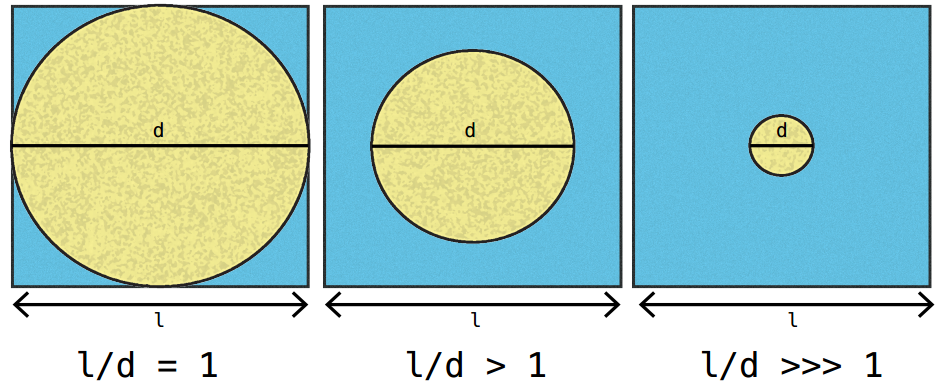
\includegraphics[width=0.6\linewidth]{ratio_lvsd.png}	
			\caption{Relation between area of circle and square}
			\label{fig::areas}
		\end{figure}
		
		From figure (\ref{fig::areas}), we have: 
		
		$ S_{circle} = \left( \dfrac{d}{2} \right)^{2} \pi$ and $ S_{square} = l^{2}$. Thus, $\pi$ can be computed as: 
		
		\begin{equation}
			\dfrac{S_{circle}}{S_{square}} = \dfrac{ \left( \dfrac{d}{2} \right)^{2} \pi}{ l^{2} }  \Rightarrow \pi 
			= 4 \left( \dfrac{l}{d} \right)^{2} \cdot \dfrac{S_{circle}}{S_{square}}
			\label{eq::pi_formular}
		\end{equation}
		
		Where  $S_{circle}$ and $S_{square}$ are the number of points that fall inside the circle and those falling outside the circle, respectively. It is important to mention that the $S_{square}$ is the total number of points generated. That is $S_{square}=$ points inside the circle $+$ points outside the circle.
		
		From the above formula, we can view the ratio $\dfrac{S_{circle}}{S_{square}}$ as a probability of any given point to fall inside the circle. Additionally, the ratio $\dfrac{l}{d} \geq = 1$ since the whole circle must be inside the square. As a result, if we were to modify the diameter of the circle, such a ratio will decrease and in the limit when $d = 0$, we have $\pi=0$: a circle whose radius is zero.
		However, changing the position of the circle –as long as it is completely contained in the square – will have no effect on the the computed value of $\pi$. But the smaller $d$ is, the more points we need for our estimation of $\pi$ to improve: many points should be computed in such a manner the whole area of the circle is full of points, which increases computational cost.
		
		%question 2
		\item
		Perform the $\pi$ estimation for 1000, 100,000 and 1,000,000 trials. Take a screenshot of these estimations and include them in your report (e.g of the python plots). What happens to the accuracy of the $\pi$ estimation when going from 1000 to 1,000,000 trials and why?
		
		We can view our equation (\ref{eq::pi_formular}) as an estimator function being multiplied by a constant $K= 4 \left( \dfrac{l}{d} \right)^{2}$, then we can rewrite (\ref{eq::pi_formular}) as: 
		\begin{equation*}
		\pi = K \dfrac{S_{circle}}{S_{square}}
		\Rightarrow
		\pi = K \cdot \sum_{i=1}^{n}{ \mathbbm{1}_{S_{circle}} (x)  } 
		\end{equation*}
		
		where $\mathbbm{1}_{S_{circle}}(x) = 1$ if the pseudo-random-generated point $x$ is inside the circle and  $\mathbbm{1}_{S_{circle}} (x)= 0$ otherwise. 
		
		The more samples we take, the more accurate our result will be. This is given by the Strong Law of Large Numbers, which states that the more samples we take from an experiment, the more the mean of these numbers will approximate the true value, that is:
		
		\begin{equation*}
		\dfrac{X_{1} + \dots + X_{n} }{n} \xrightarrow[{ }]{\text{a.s}} \mu \text{ as } n \rightarrow \infty
		\end{equation*}
		Where $X_{1} + \dots + X_{n}  $ is the sum of our indicator function over $n$ samples. 
		
		that is (such a mean will be the true value with probability 1), 
		
		\begin{equation*}
		\mathbbm{P}\left( \lim_{n\rightarrow \infty} \dfrac{S_{n}}{n} = \mu \right) = 1
		\end{equation*}
		
		with $S_{n} = X_{1} + \dots + X_{n}$. The error rate of our estimator is given by the Central Limit Theorem. Then, the error in our Monte Carlo estimation of $\pi$ decays at a rate $1/ \sqrt{N}$ ($N$ is the number of samples): 
		
		\begin{equation*}
		\dfrac{S_{n} - n\mu }{ \sigma \sqrt{n} }
		\xrightarrow[{ }]{\text{d}} Y \sim \mathcal{N}(0, 1)
		\text{ as } n \rightarrow \infty
		\end{equation*}
		
		with $\sigma^2$ the variance of $S_{n}$. Hence, we have the following plots for different number of samples:
		
		\begin{figure}[H]
			\centering
			\begin{subfigure}[b]{0.37\linewidth}
				\centering
				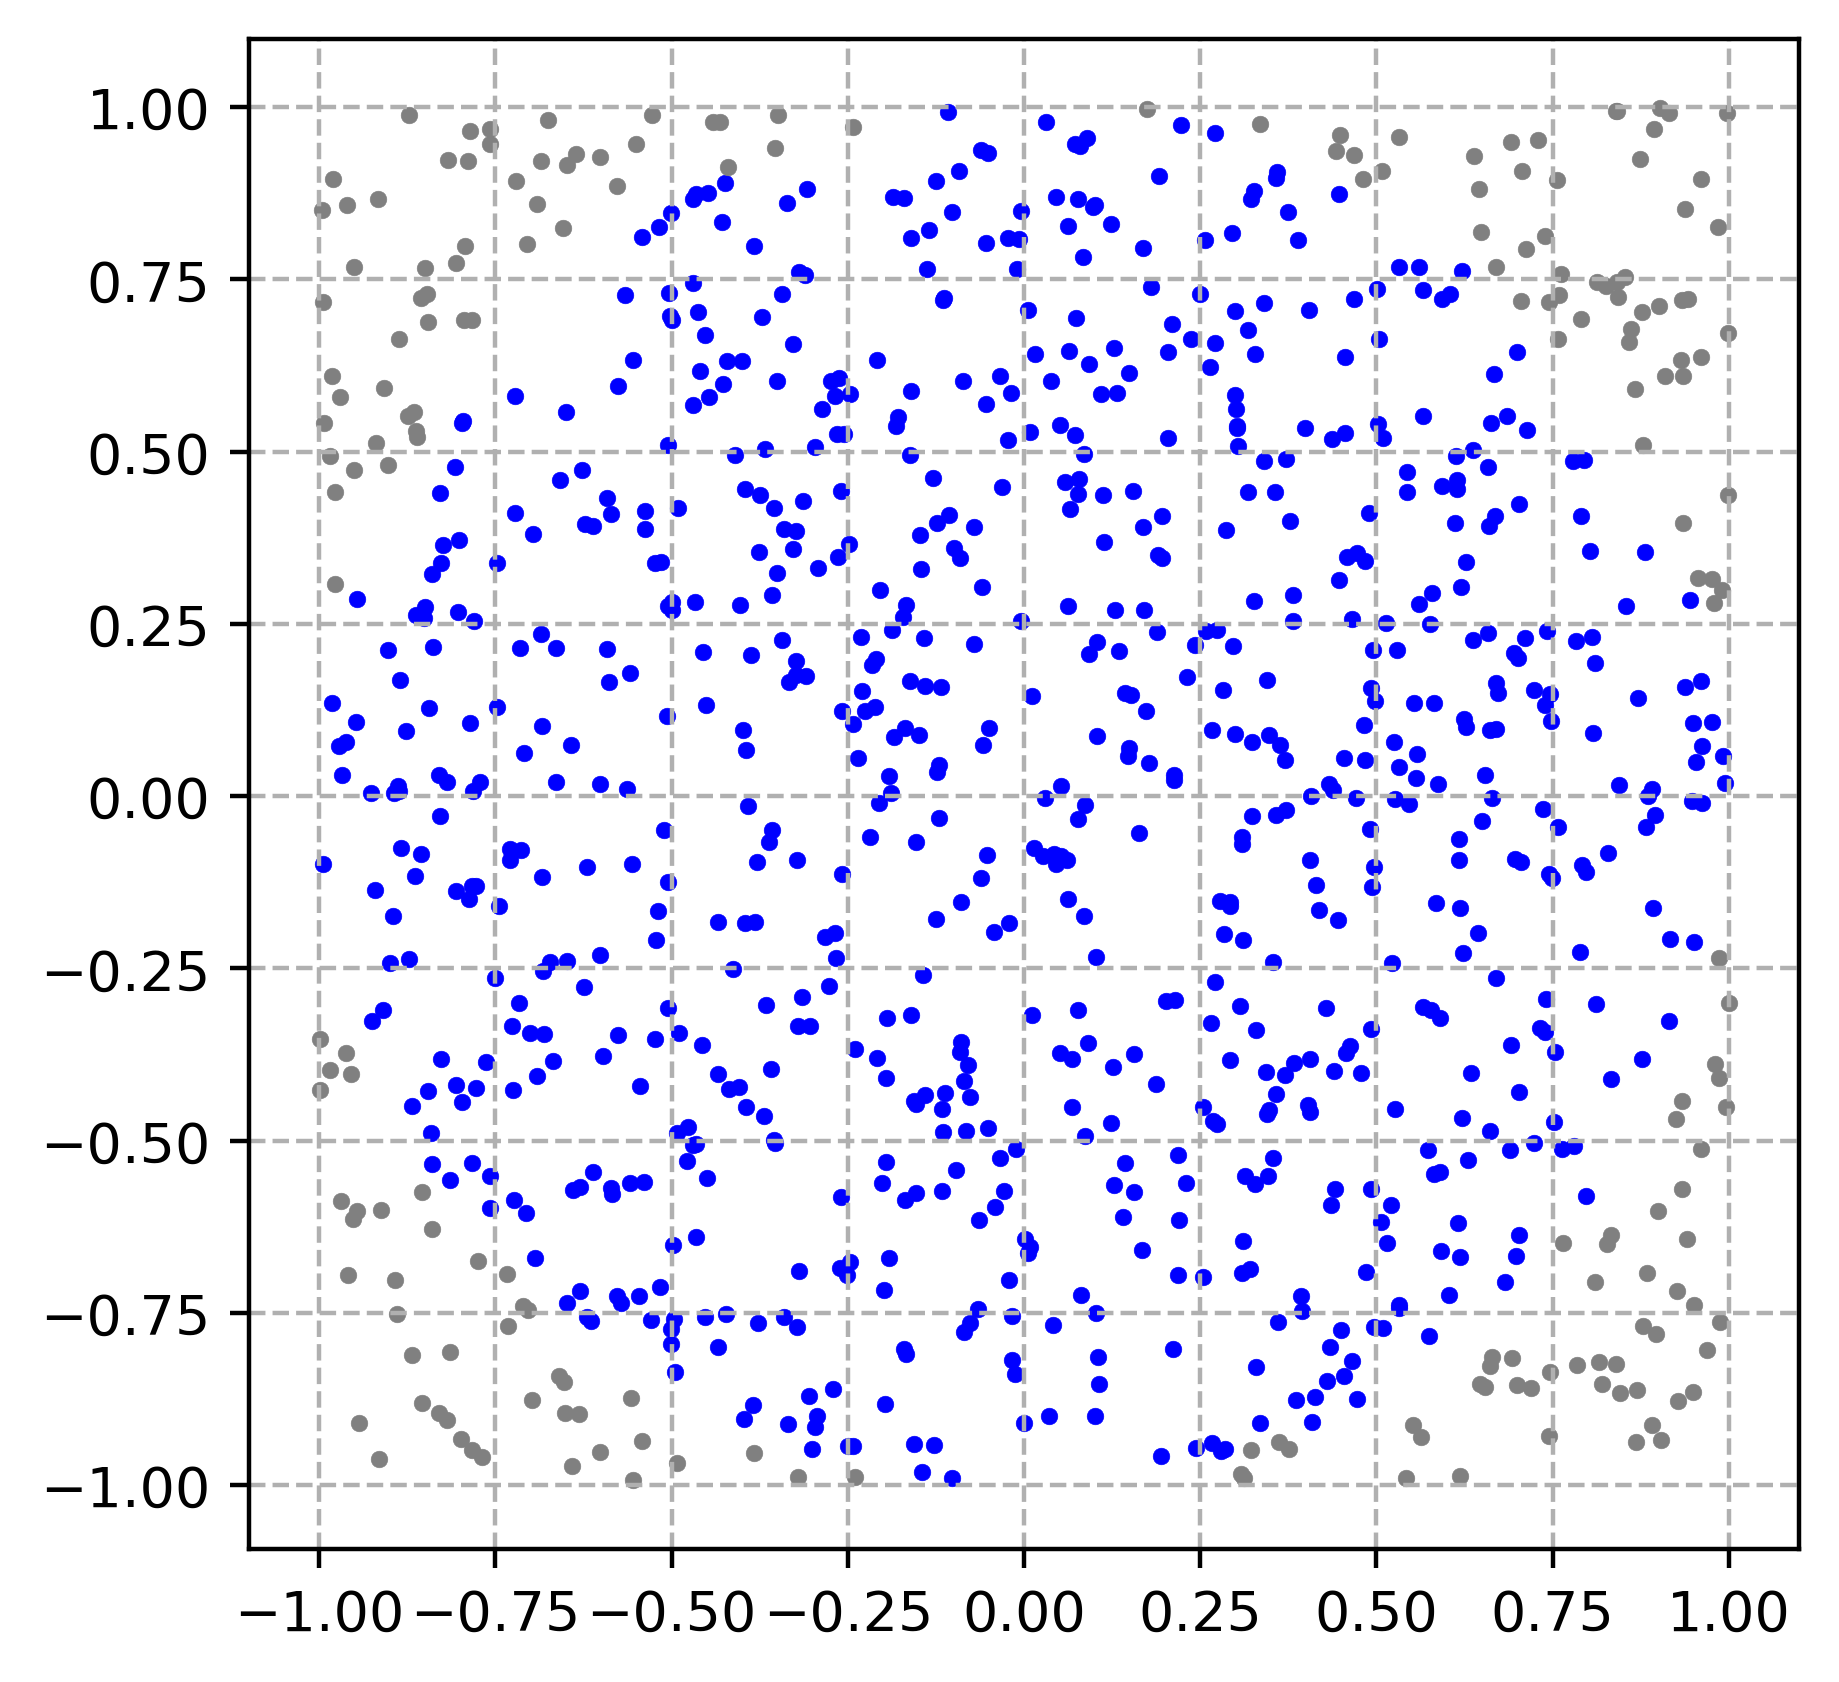
\includegraphics[width=\linewidth]{oneThousandnSamples.png}
				\caption{1000 points, $\pi=3.18$.}
			\end{subfigure}		
			\hfill
			\begin{subfigure}[b]{0.37\linewidth}
				\centering
				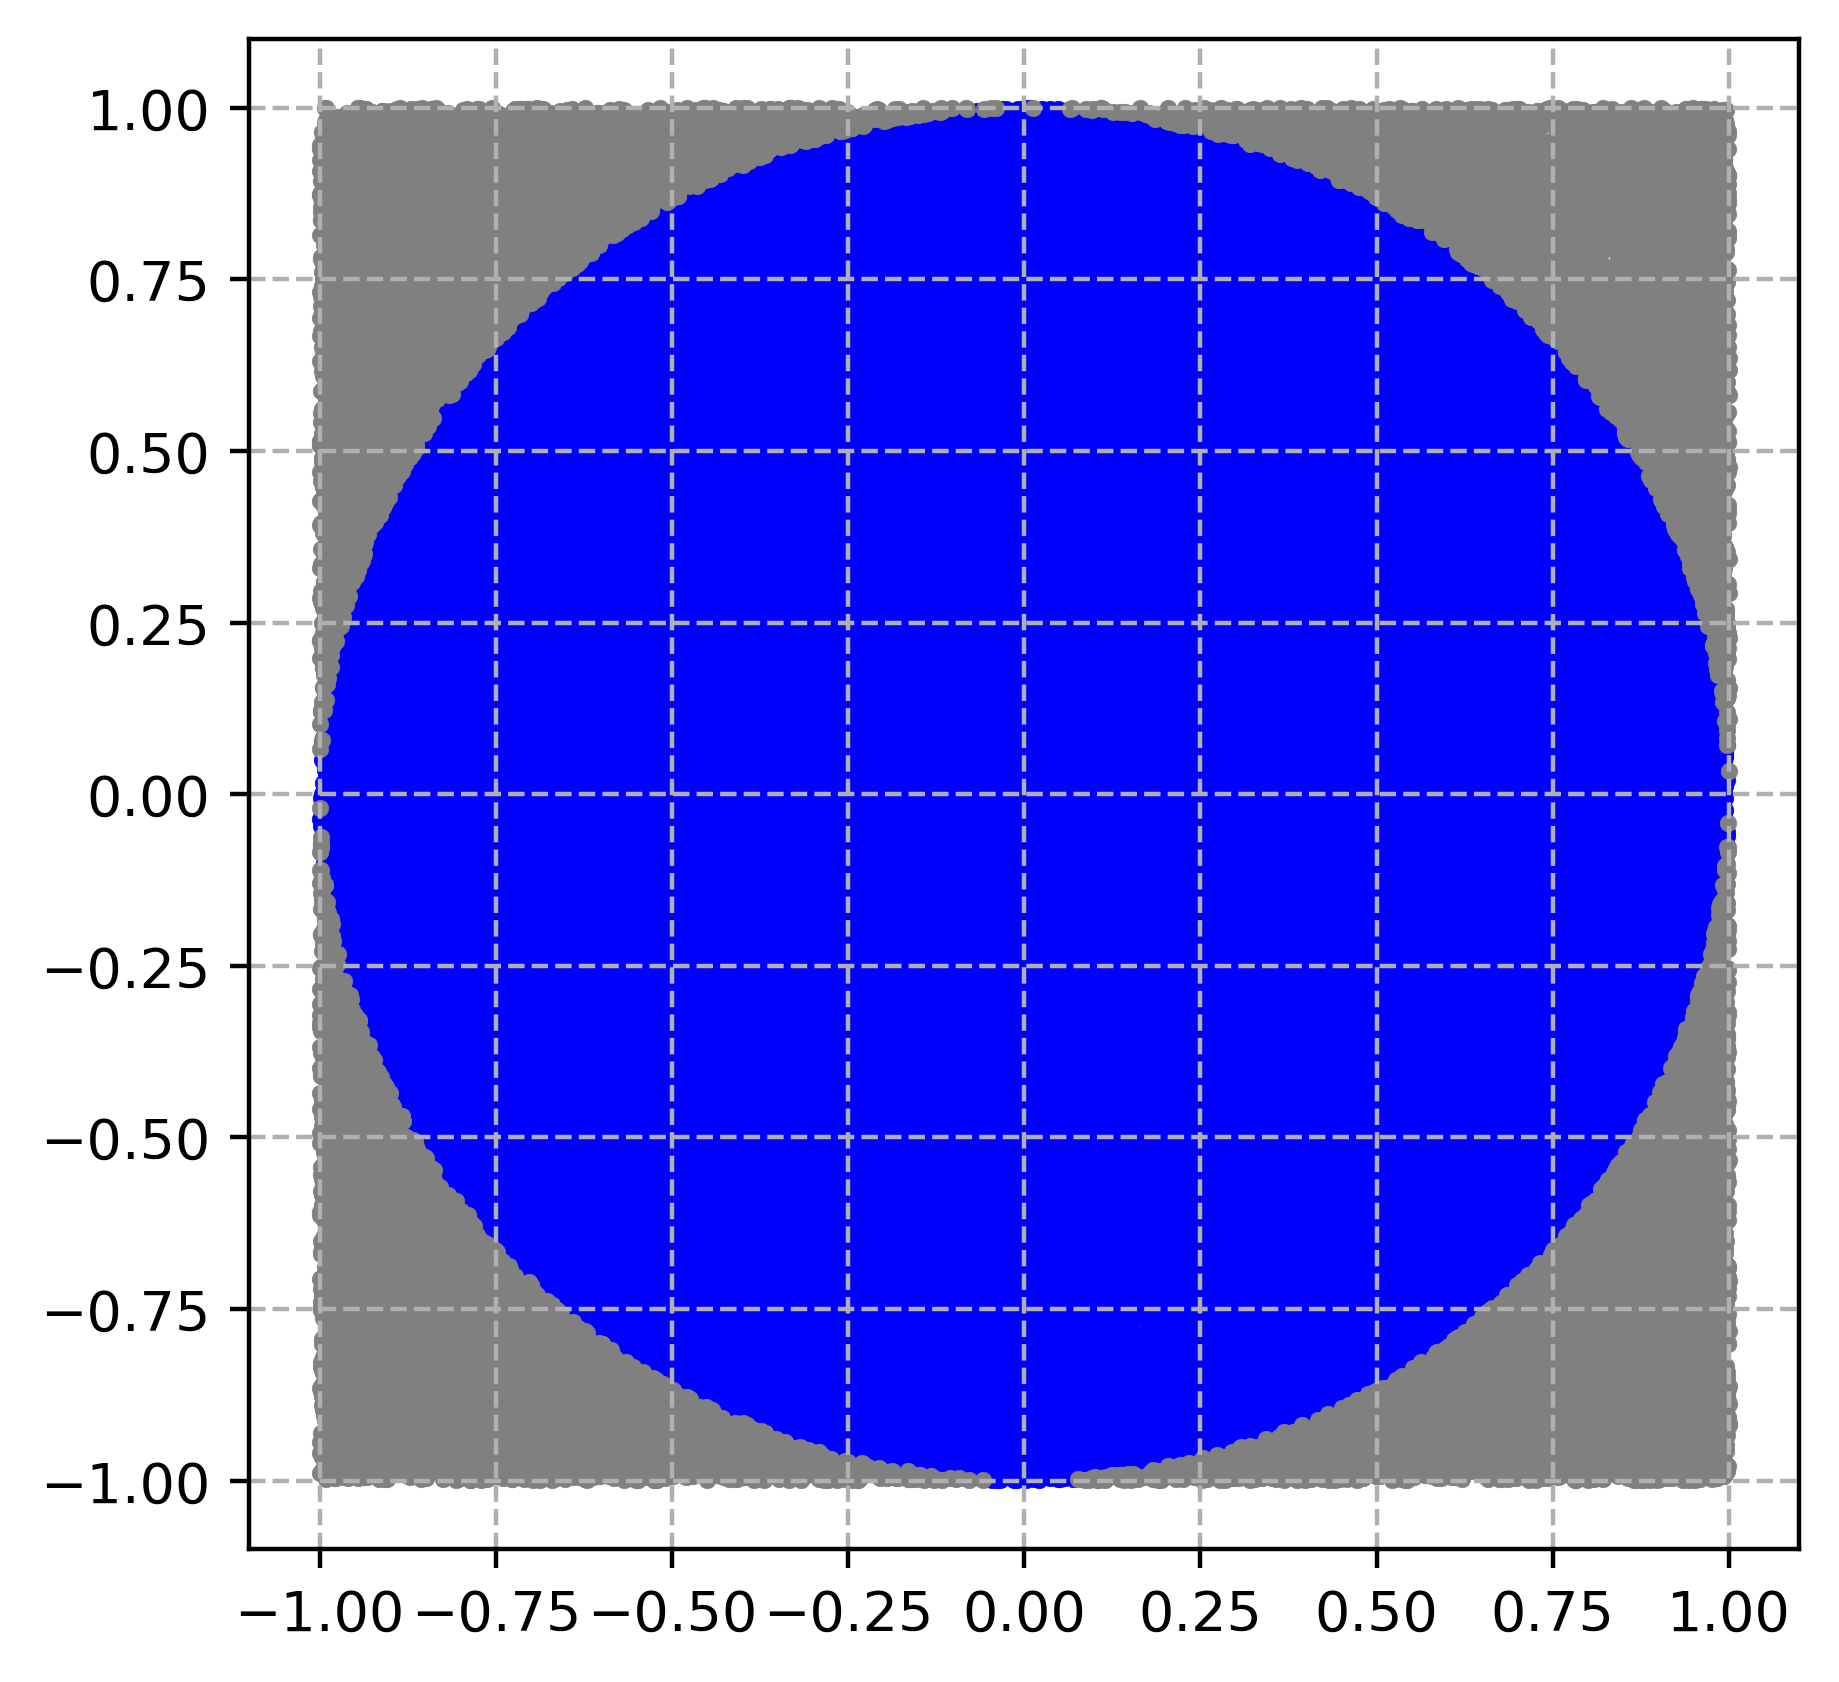
\includegraphics[width=\linewidth]{hundredthousandSamples.png}
				\caption{100000 points, $\pi = 3.13968$.}
			\end{subfigure}		
			\begin{subfigure}[b]{0.37\linewidth}
				\centering
				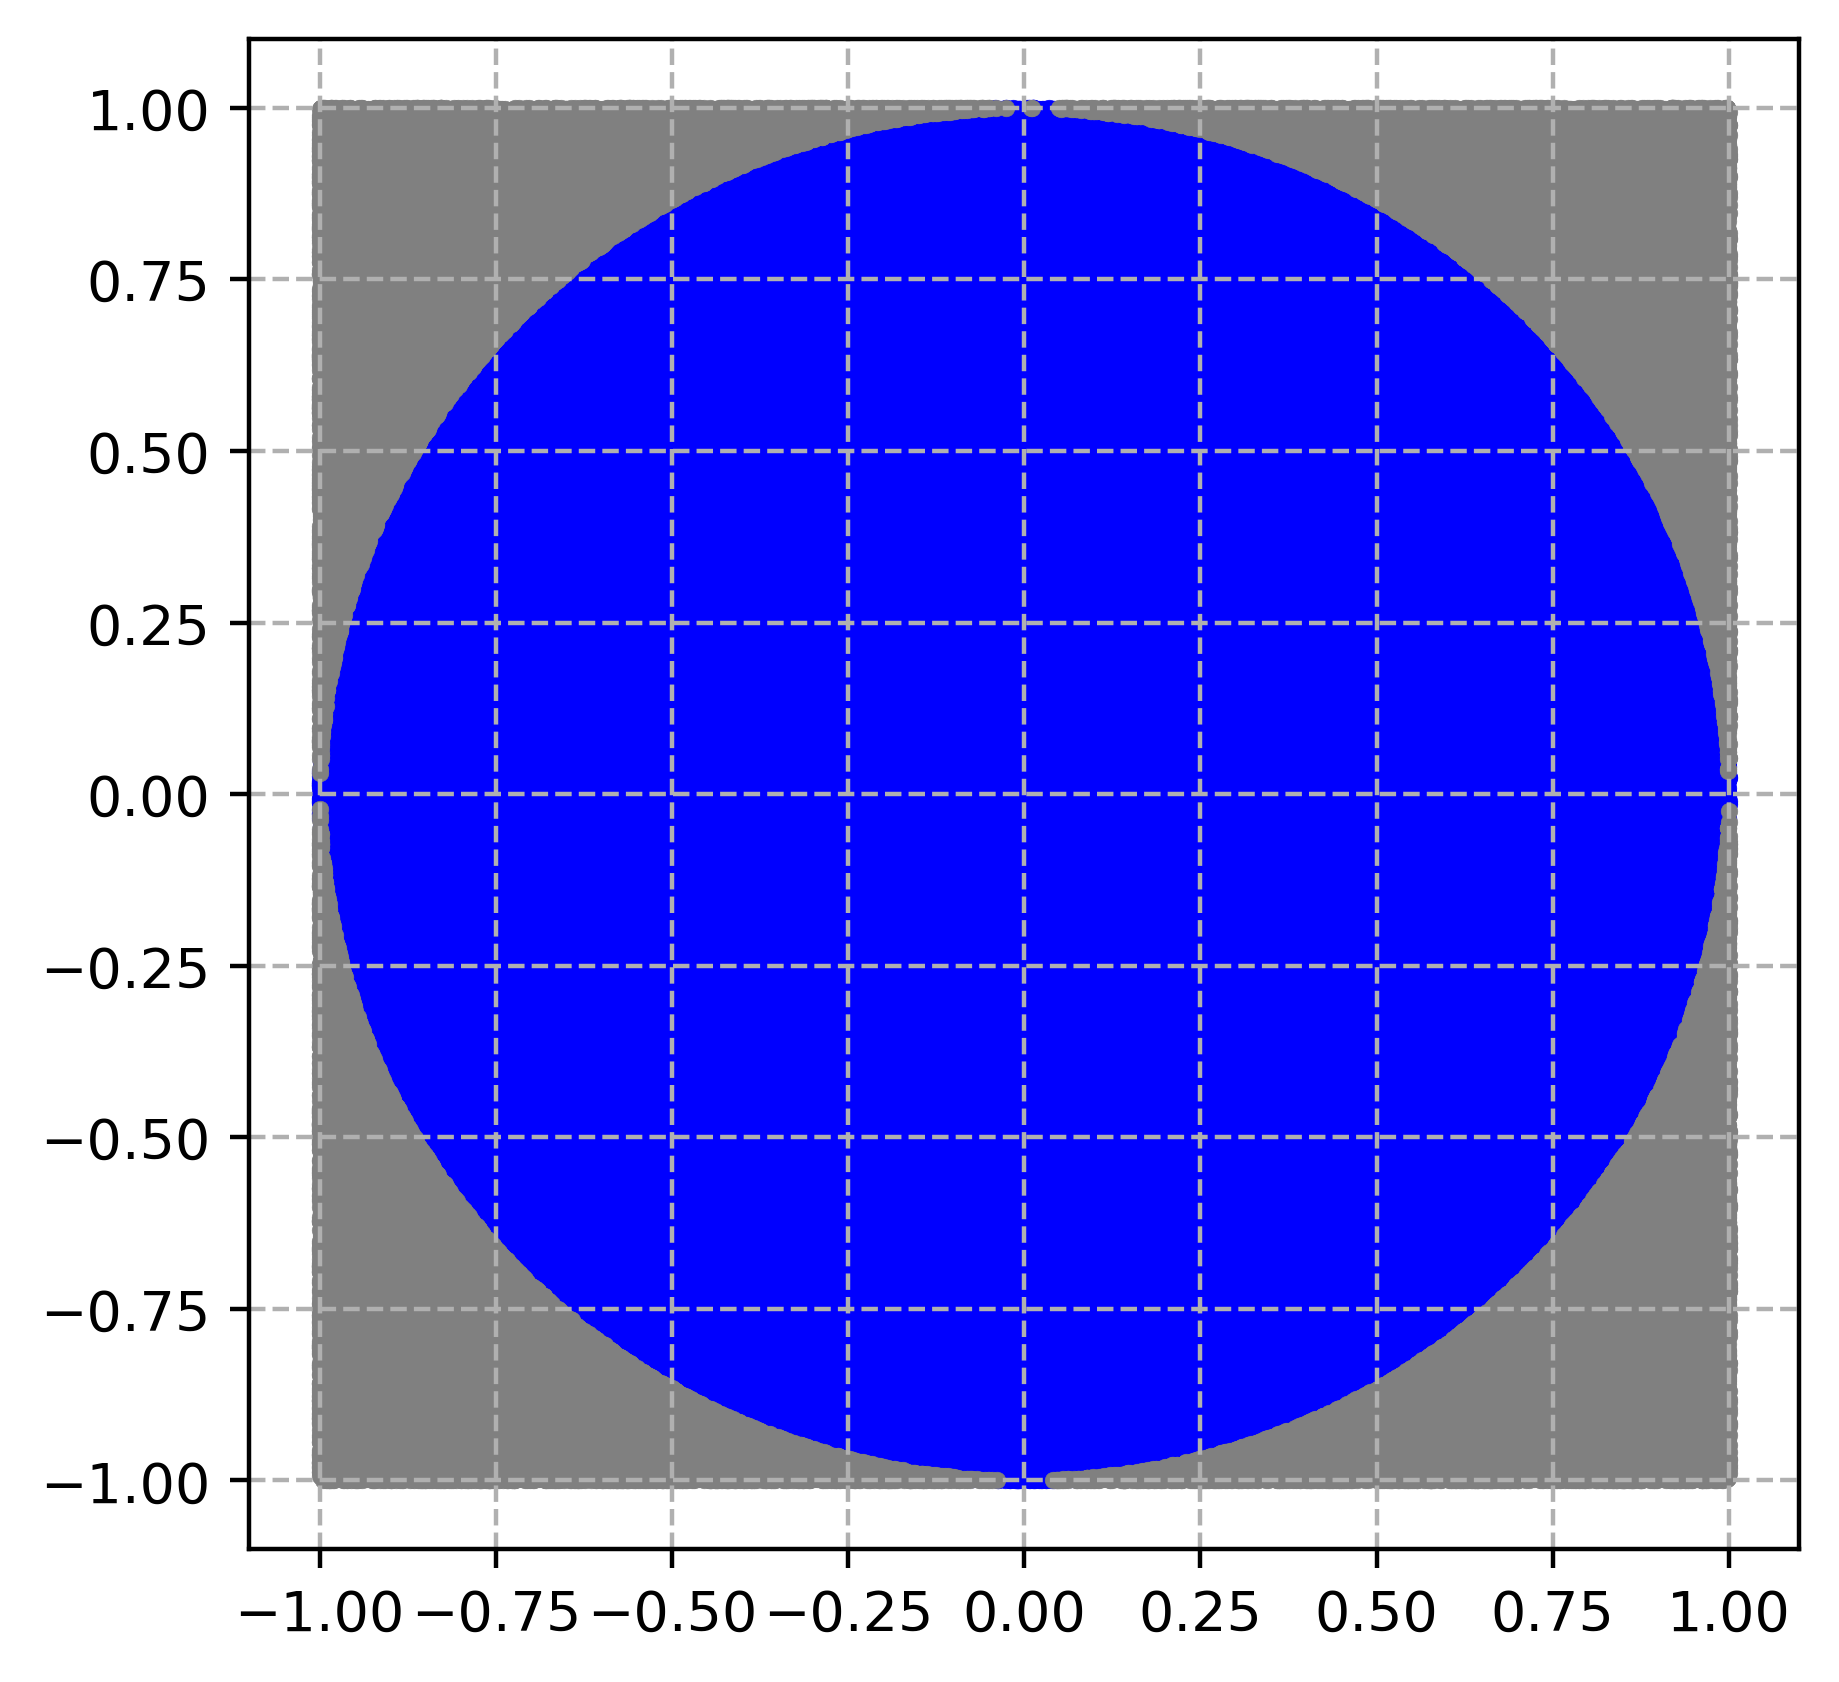
\includegraphics[width=\linewidth]{millionSamples.png}
				\caption{1000000 points, $\pi=3.14012$.}
			\end{subfigure}		
			\caption{$\pi$ estimation for different number of points.}
			\label{fig::que2_pi}
		\end{figure}    
		
		For each of the above figures the probabilities of finding a point inside the circle are 0.795  , 0.78492 and 0.78503, respectively. Besides, the errors with respect to the true value $\pi$ are 3.57367822e-07, 3.57367822e-09 and 3.57367822e-10 for each figure.  	
		
		%question 3
		\item
		What happens if you use the same seed for the PRNG?
		
		If we set the seed for the PRNG, the sequence of pseudo-random numbers starts at the same value and then we obtain the same sequence for each run of our program, which means our results will be always the same after running our code over and over again for a given number of samples.
		However, we must set such a seed every time we call the random number generator function. Since we  called the seed function once at the very beginning of the program, it has no effect on our results.
		
		It is worth pointing out that setting or not the seed will have no effect on the $\pi$ estimation that we compute since the random numbers are generated in such a manner that we can think of them as identical and independent distributed, i.i.d for short. 
		
		We ran our program setting the seed to 42.
		
		%question 4
		\item What happens to the estimation of $\pi$ when the circle origin is changed? Why?

		As long as the whole area of the circle is inside the square, the center of the circle has no effect on the $\pi$ estimation. This happens since we are counting the number of points inside of the circle, then its center has no importance. Furthermore, our function for estimating $\pi$ does not depend on the center of the circle at all. Besides, the used random numbers are iid; as result, each point has the same probability of falling inside the circle.
		
		To illustrate the latter, we have the following plots for two distinct locations of the center of the circle. For such plots, the radius of the circle is equal to $0.50 \cdot l$, by doing so we could have all its area inside the square. We compute $\pi$ for 10000, 20000 and 30000 samples; hence we have: 
		
		\begin{figure}[H]
		\centering
		\begin{subfigure}[b]{0.32\linewidth}
			\centering
			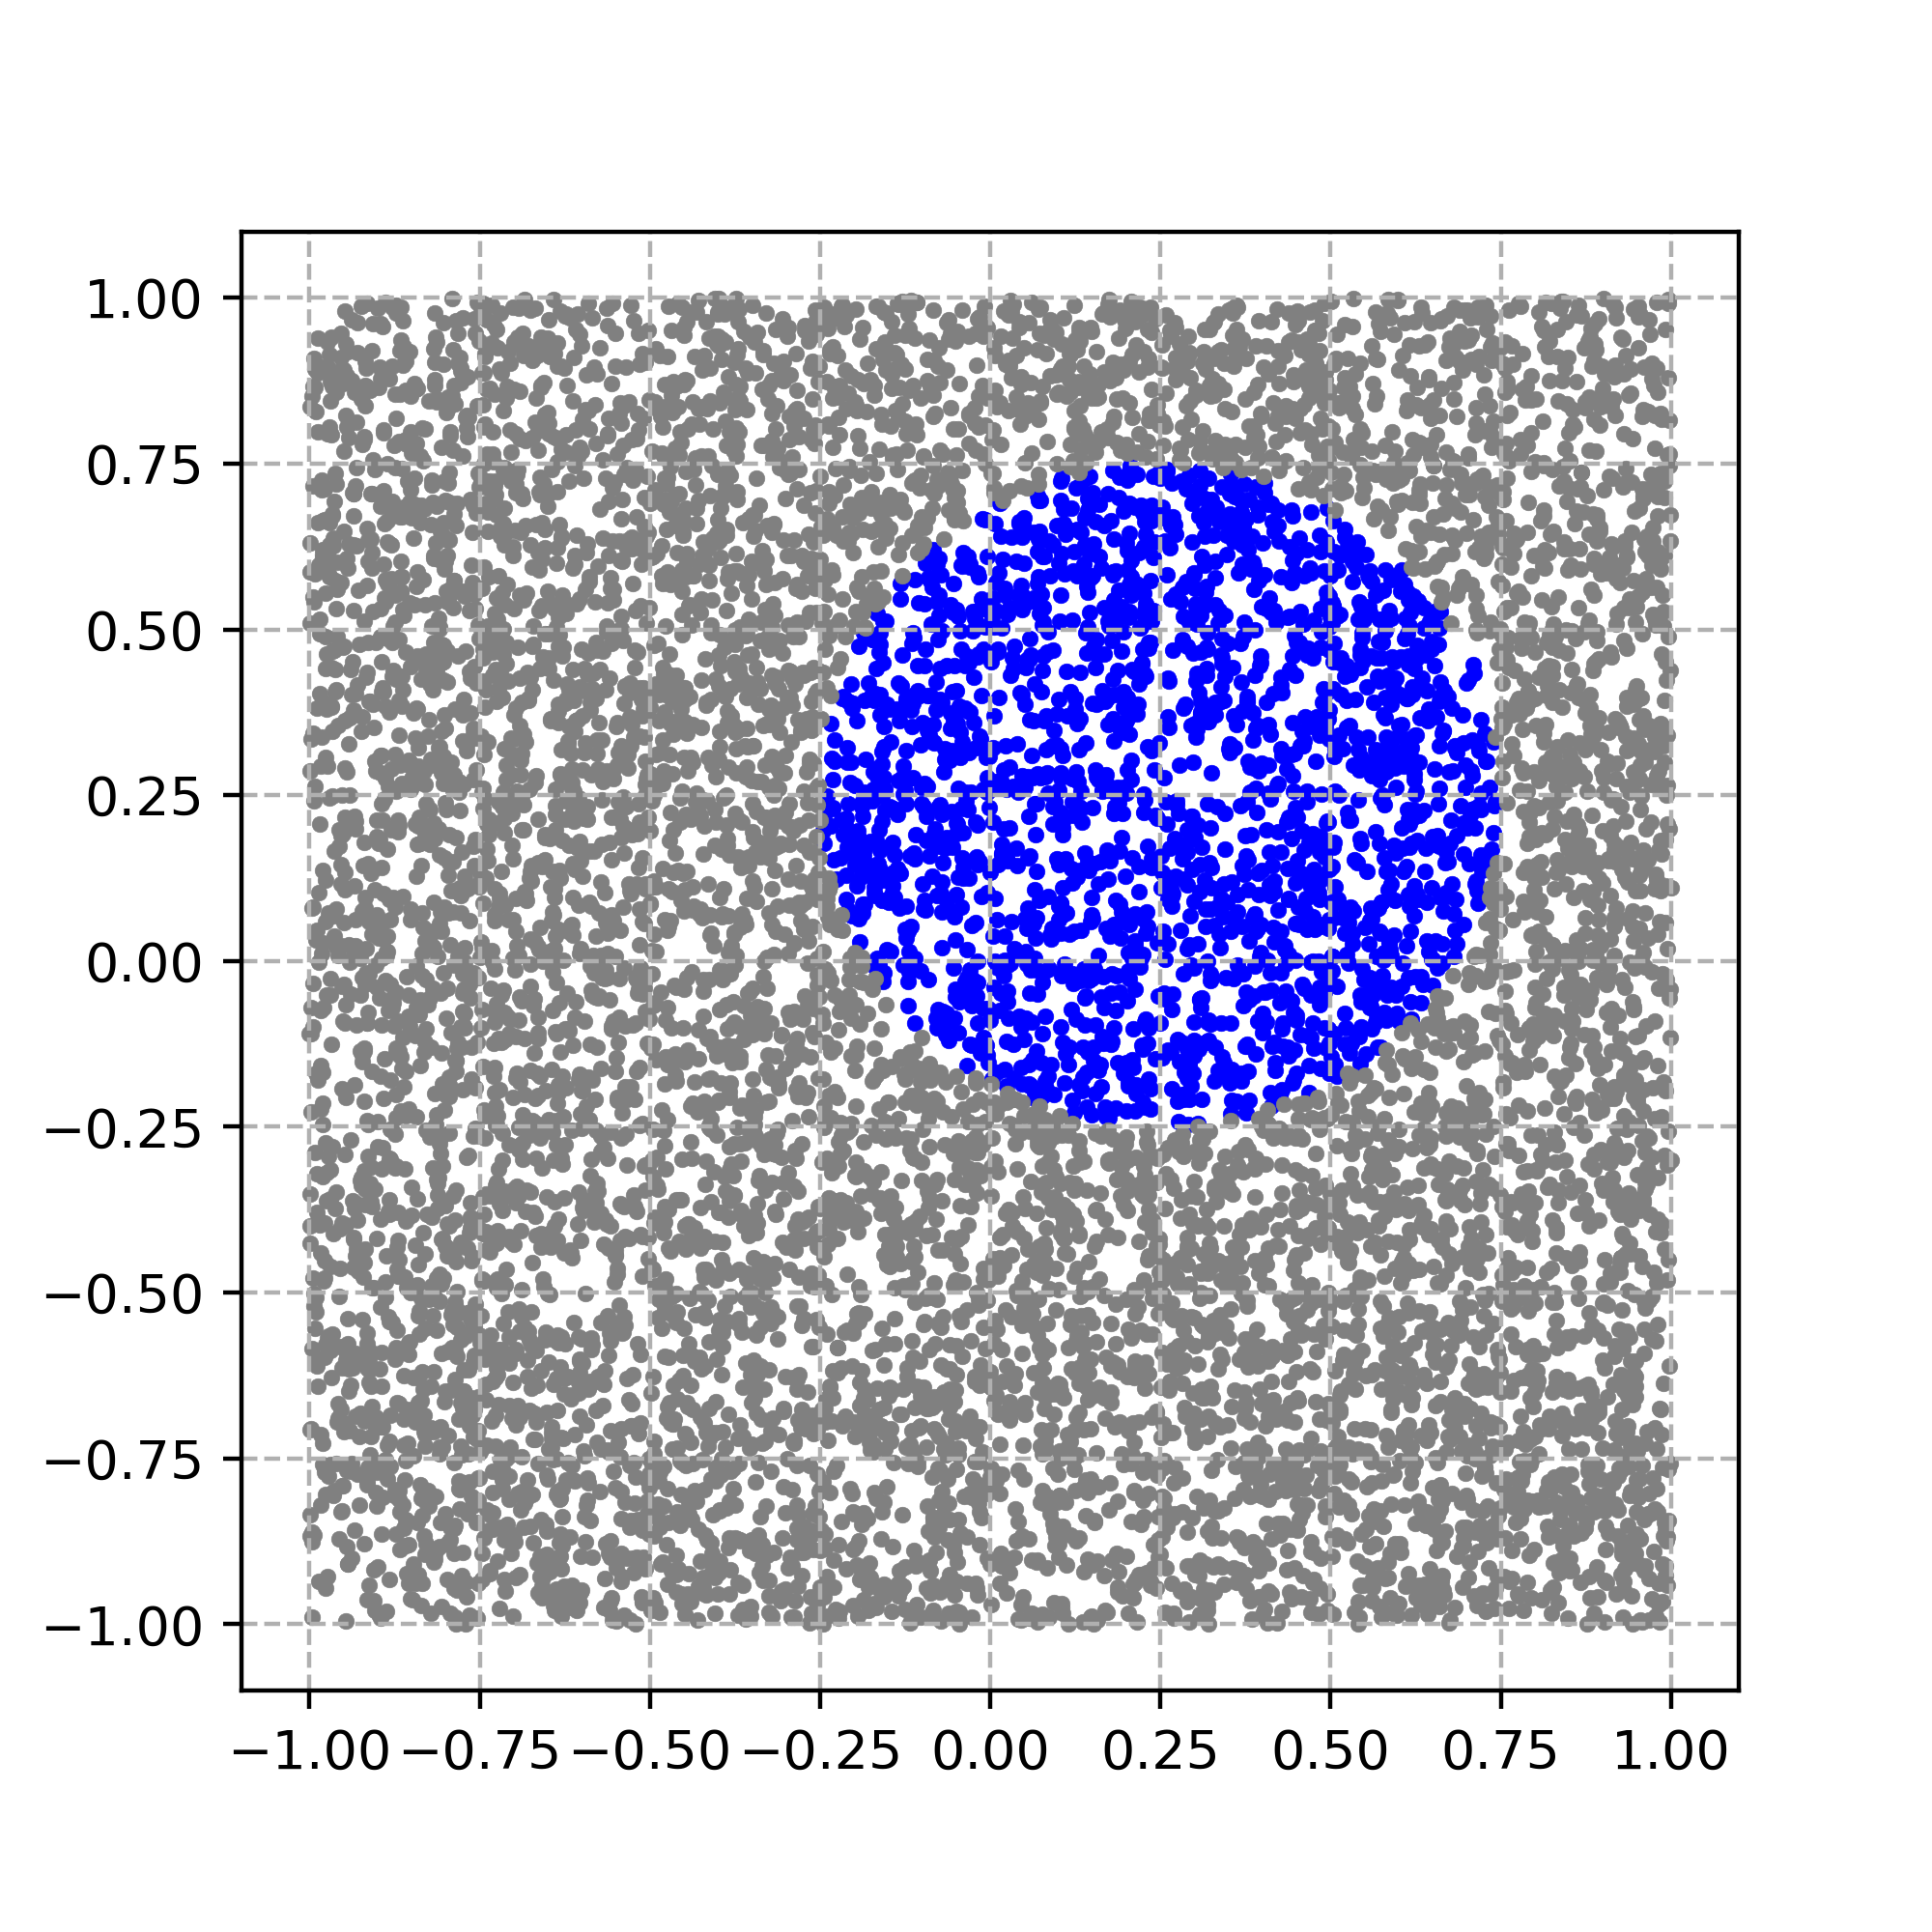
\includegraphics[width=\linewidth]{estimation4_10000.png}
			\caption{10000 points, $\pi=3.1504$.}
		\end{subfigure}	
		\hfill			
		\begin{subfigure}[b]{0.32\linewidth}
			\centering
			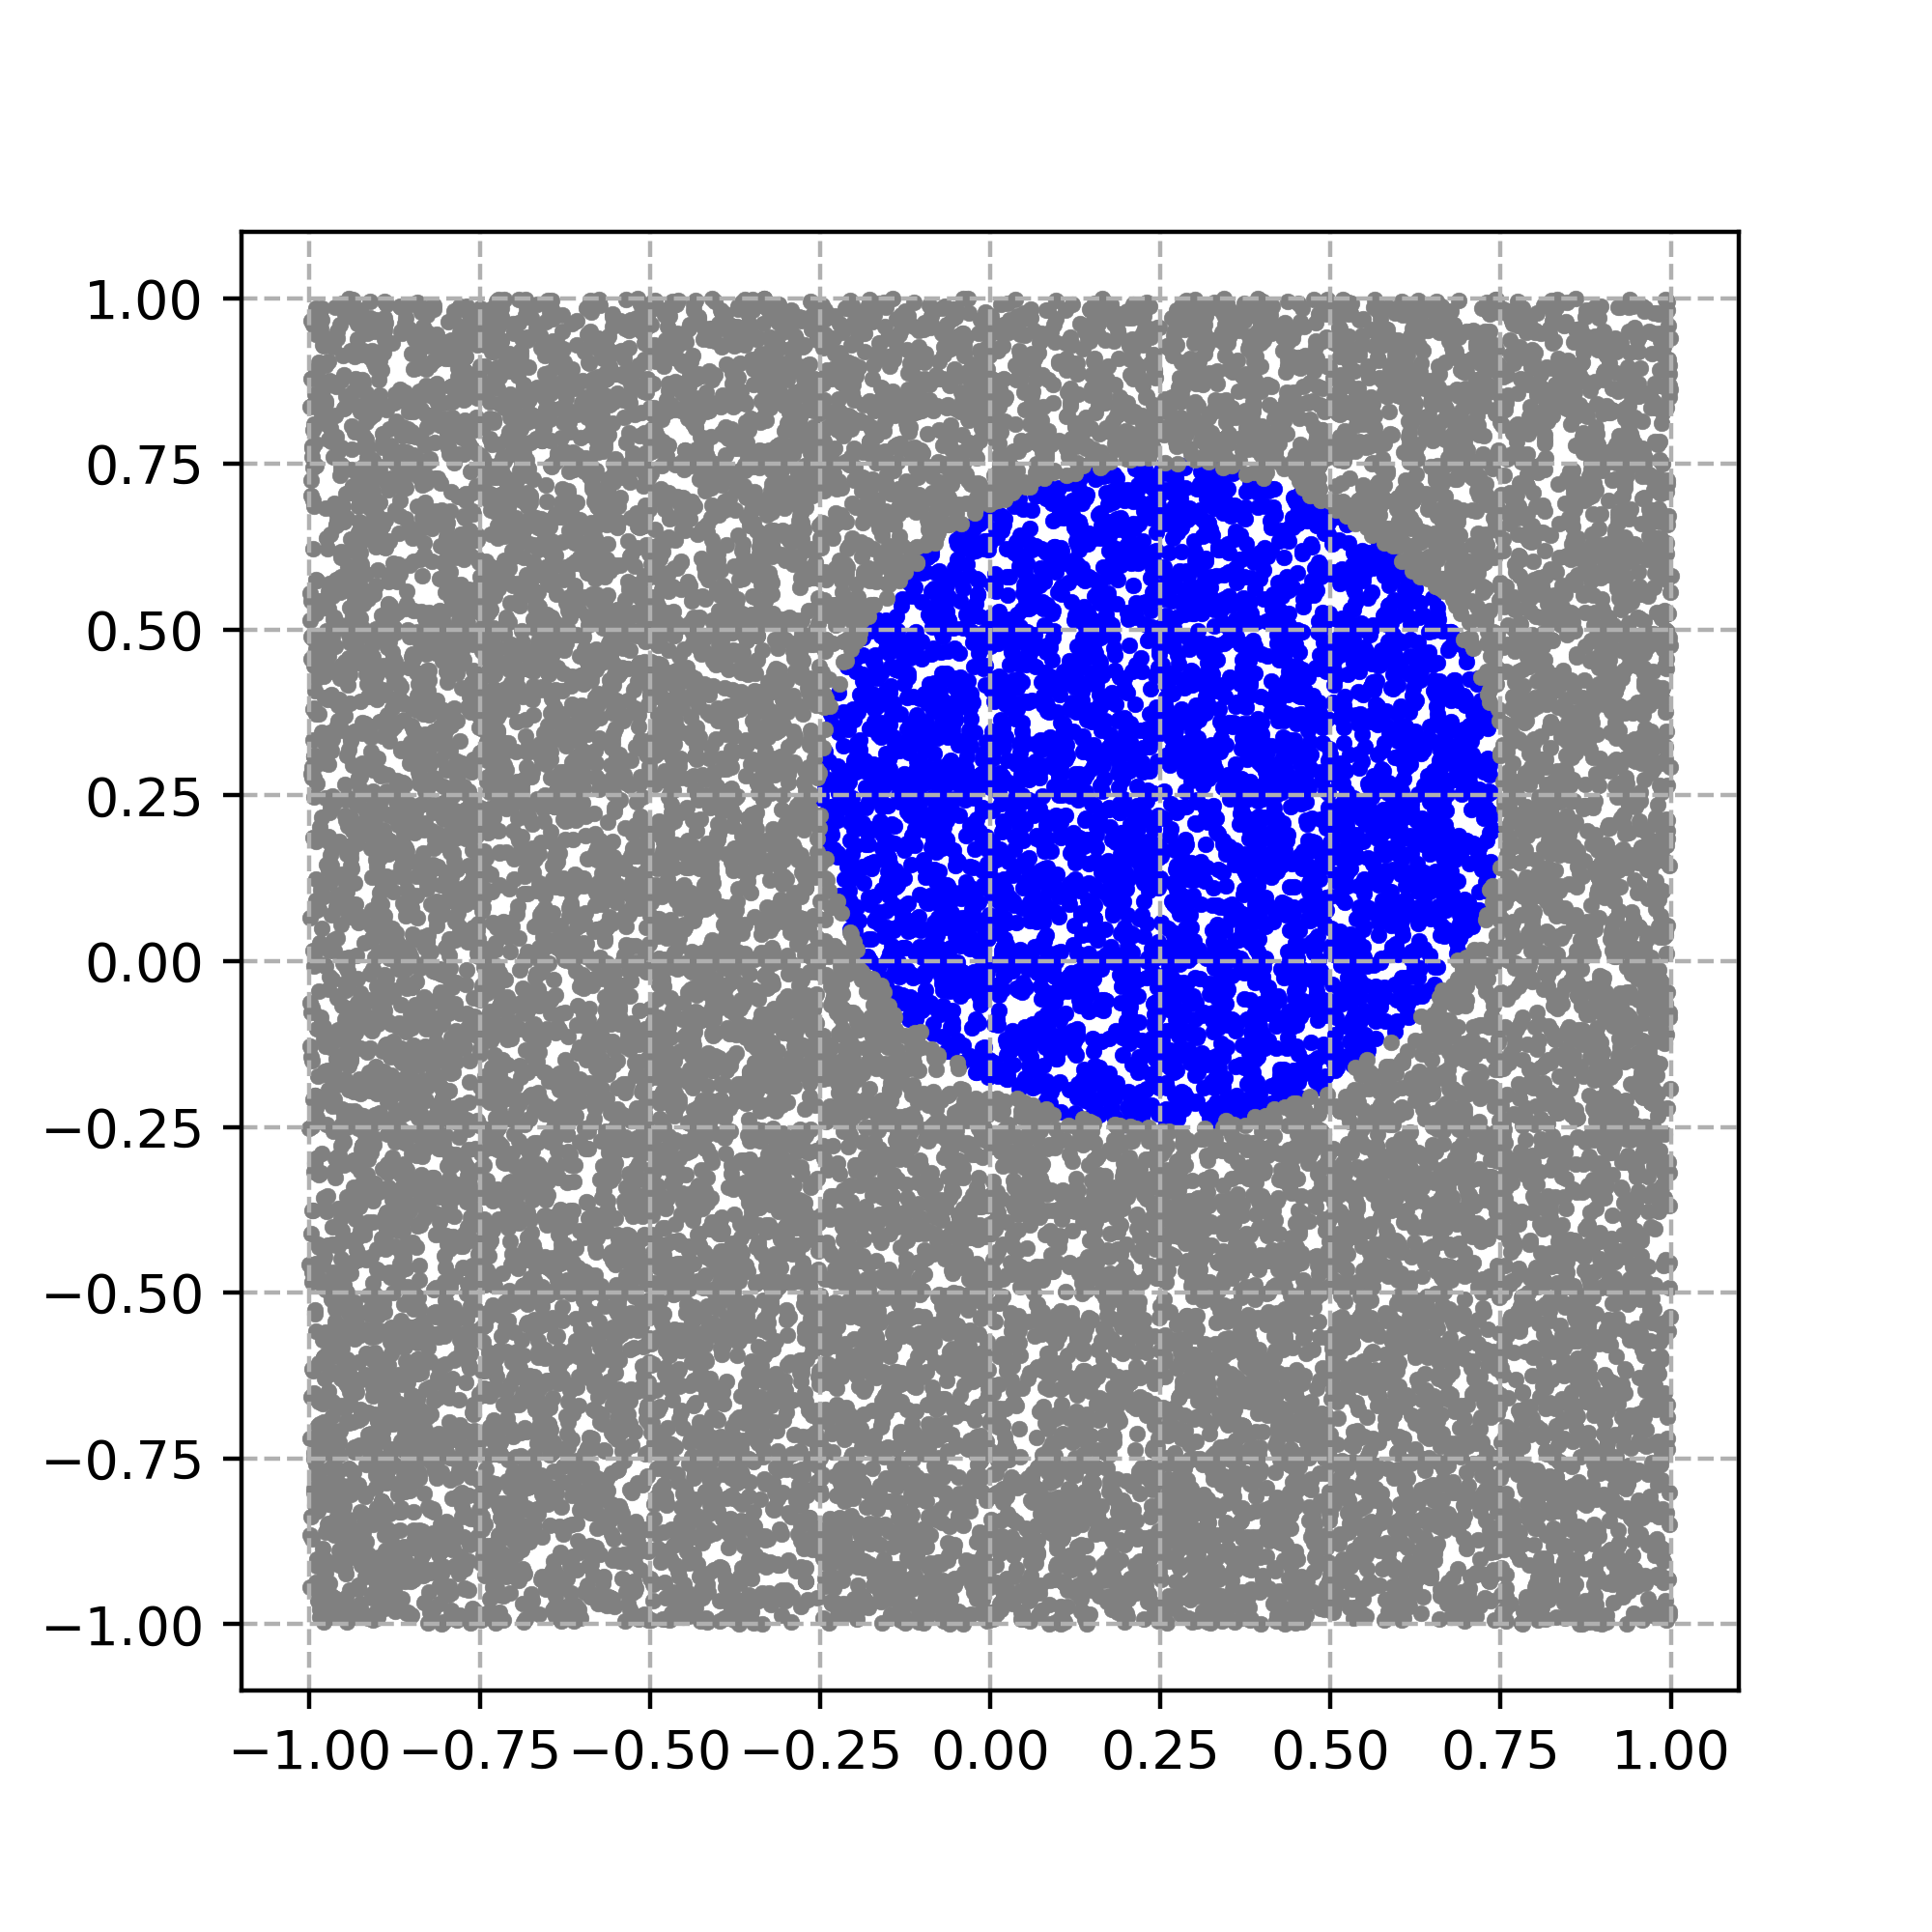
\includegraphics[width=\linewidth]{estimation4_20000.png}
			\caption{20000 points, $\pi = 3.1064$.}
		\end{subfigure}		
		\hfill
		\begin{subfigure}[b]{0.32\linewidth}
			\centering
			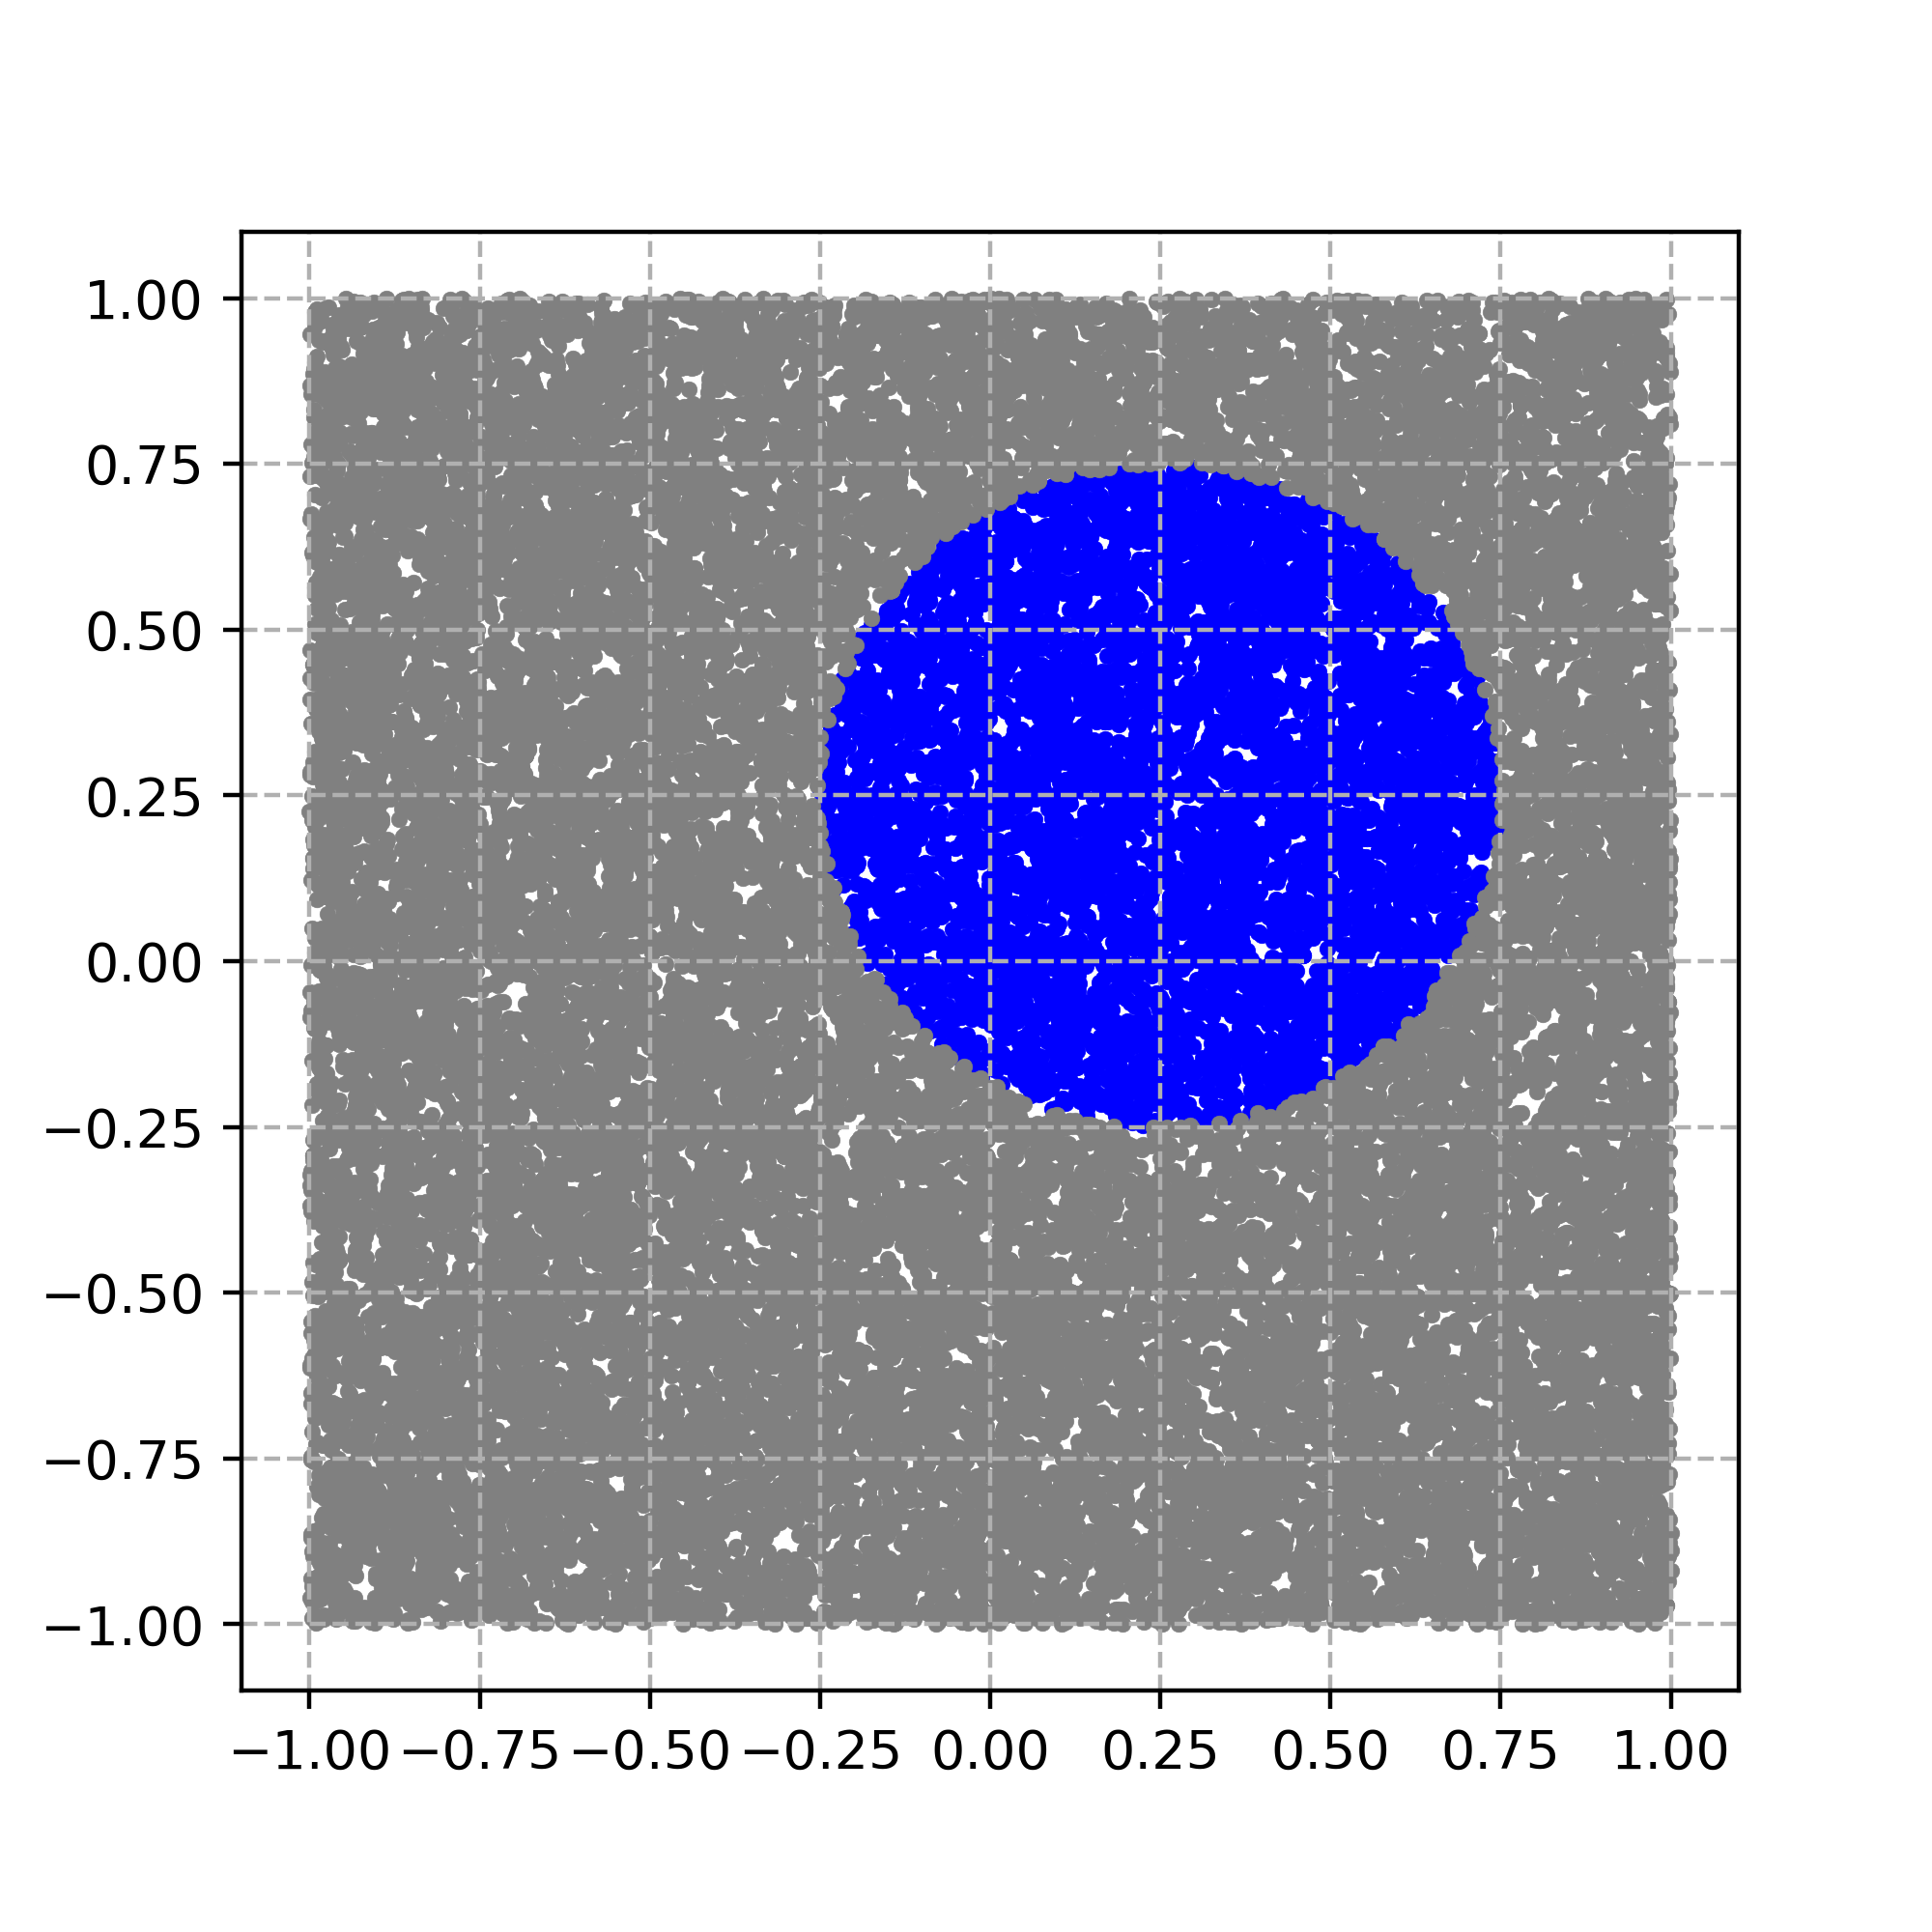
\includegraphics[width=\linewidth]{estimation4_30000.png}
			\caption{30000 points, $\pi= 3.13066667$.}
		\end{subfigure}		
		\caption{$\pi$ estimation changing center of the circle, 1.}
		\label{fig::que4_1}
		\end{figure}    	

		\begin{figure}[H]
			\centering
			\begin{subfigure}[b]{0.32\linewidth}
				\centering
				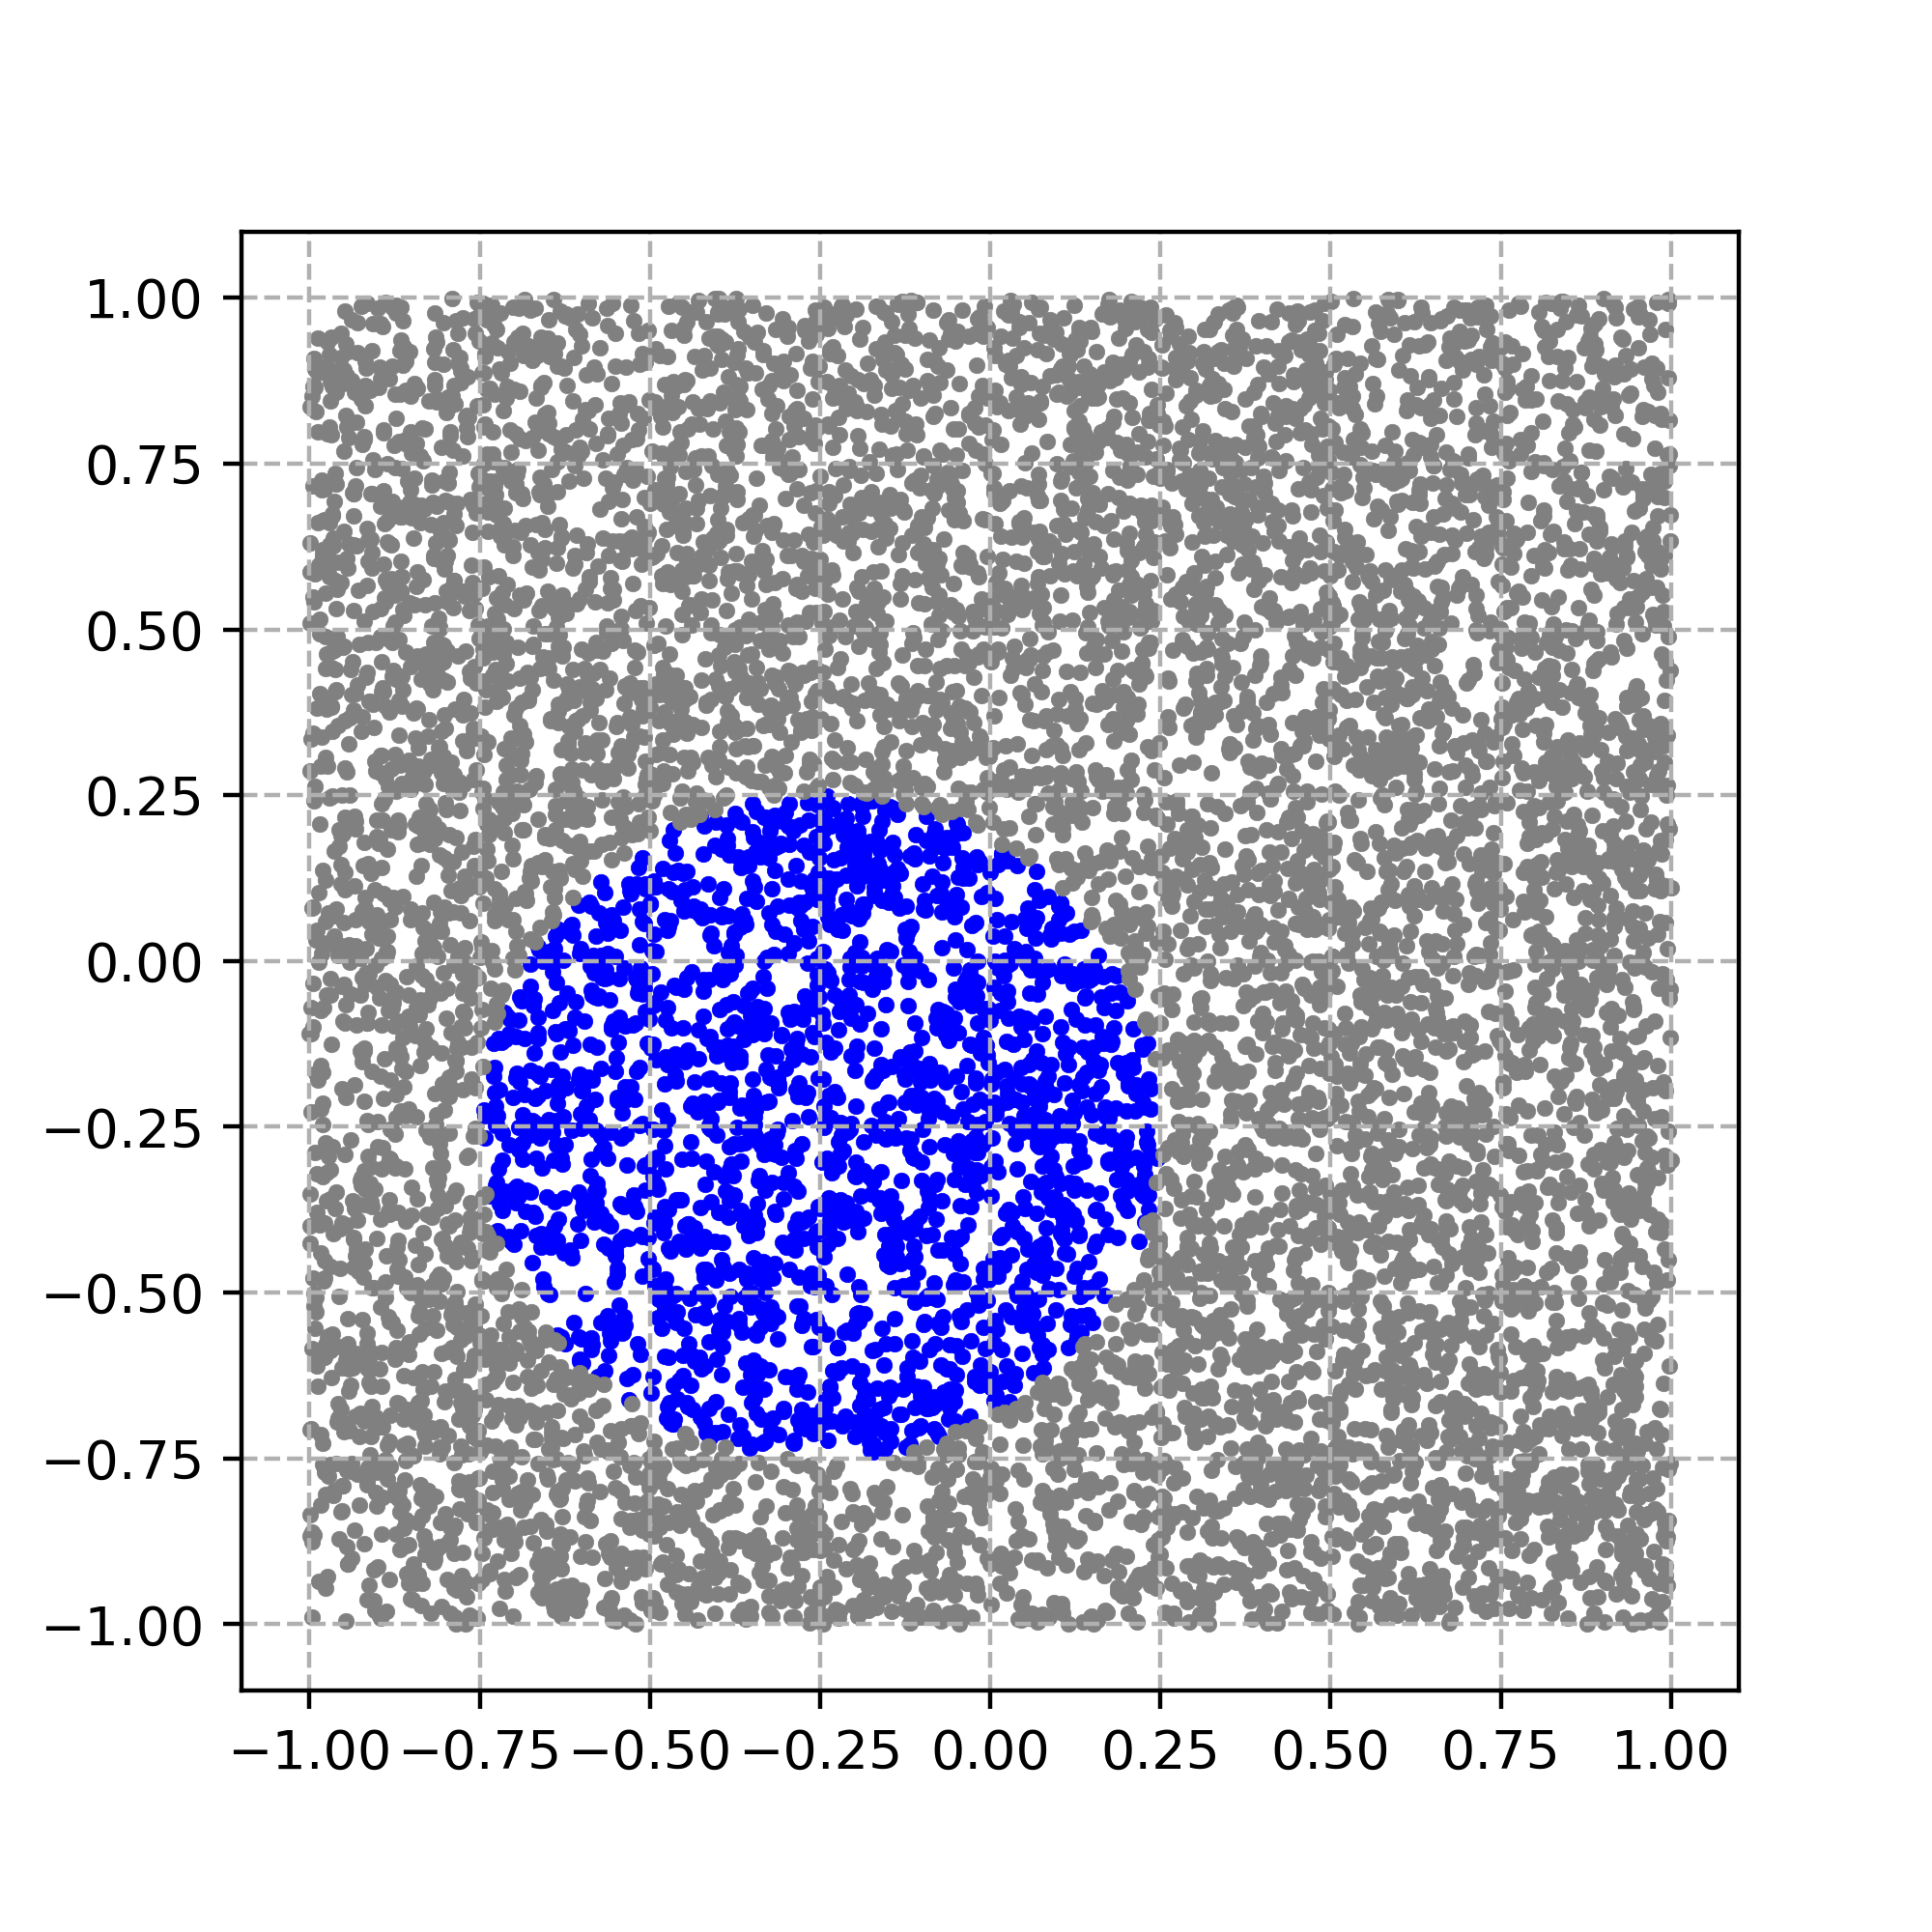
\includegraphics[width=\linewidth]{estimation4_2_10000.png}
				\caption{10000 points, $\pi=3.056$.}
			\end{subfigure}		
			\hfill
			\begin{subfigure}[b]{0.32\linewidth}
				\centering
				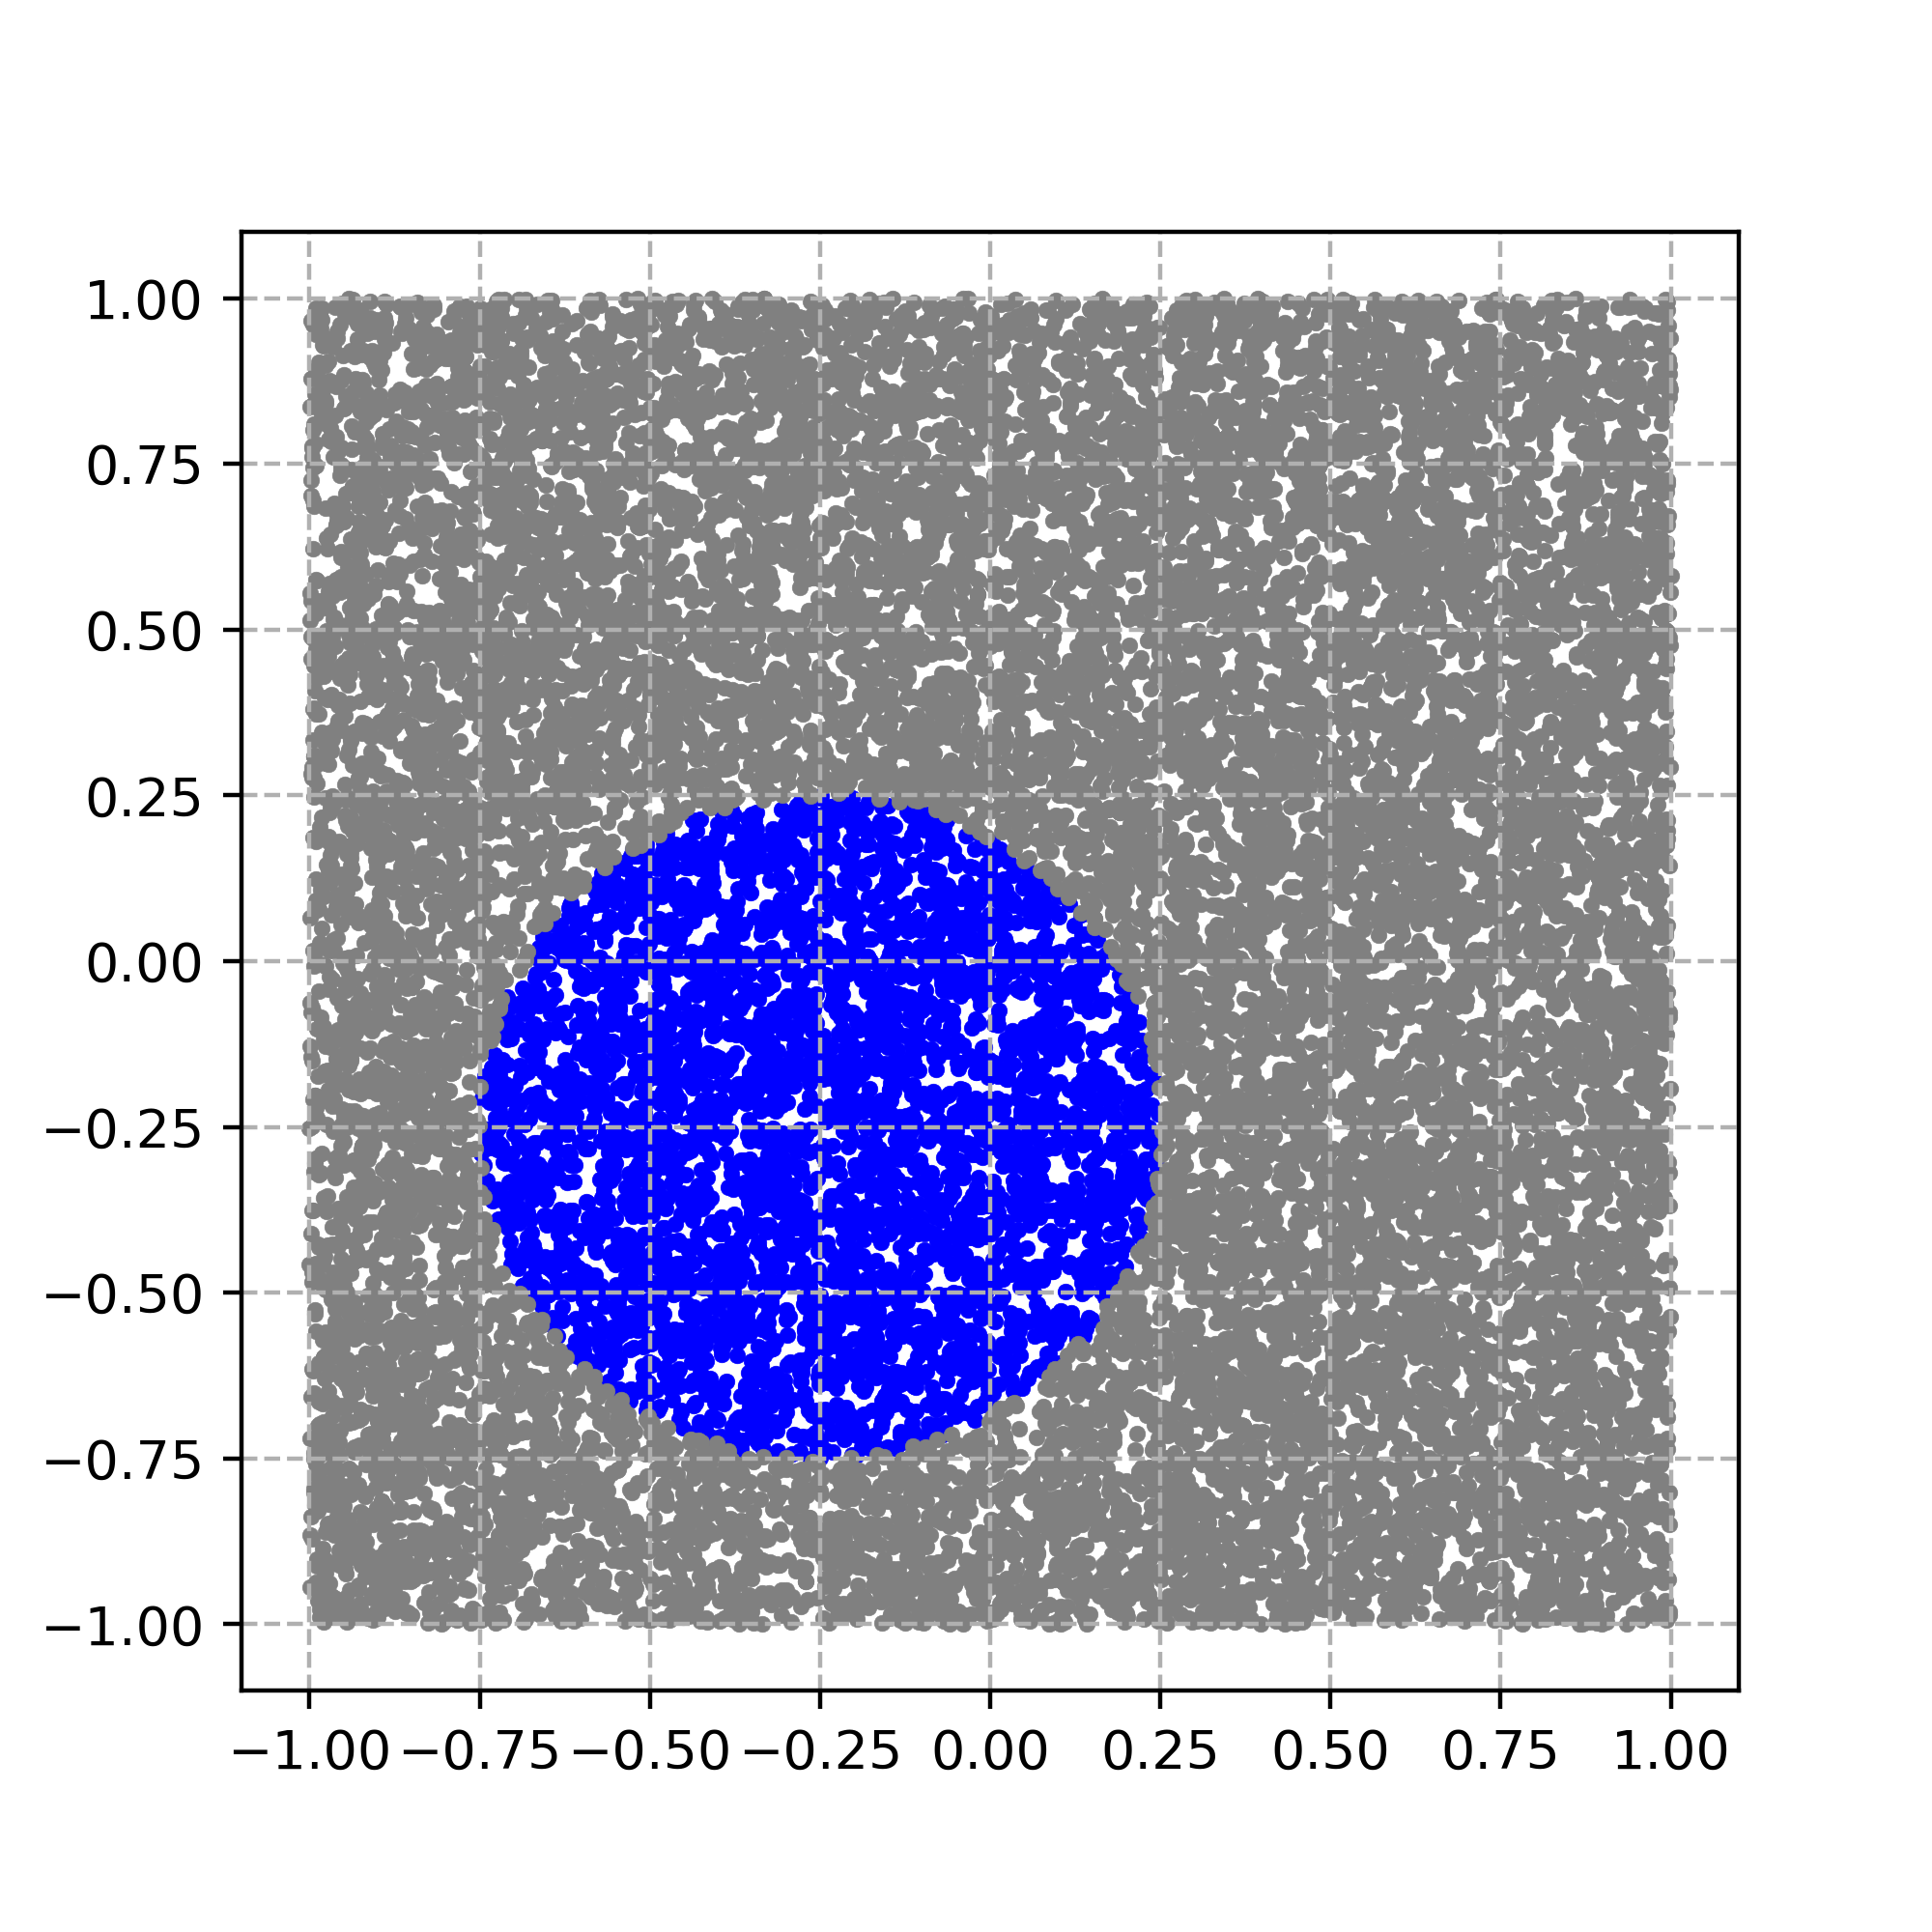
\includegraphics[width=\linewidth]{estimation4_2_20000.png}
				\caption{20000 points, $\pi = 3.1816$.}
			\end{subfigure}
			\hfill
			\begin{subfigure}[b]{0.32\linewidth}
				\centering
				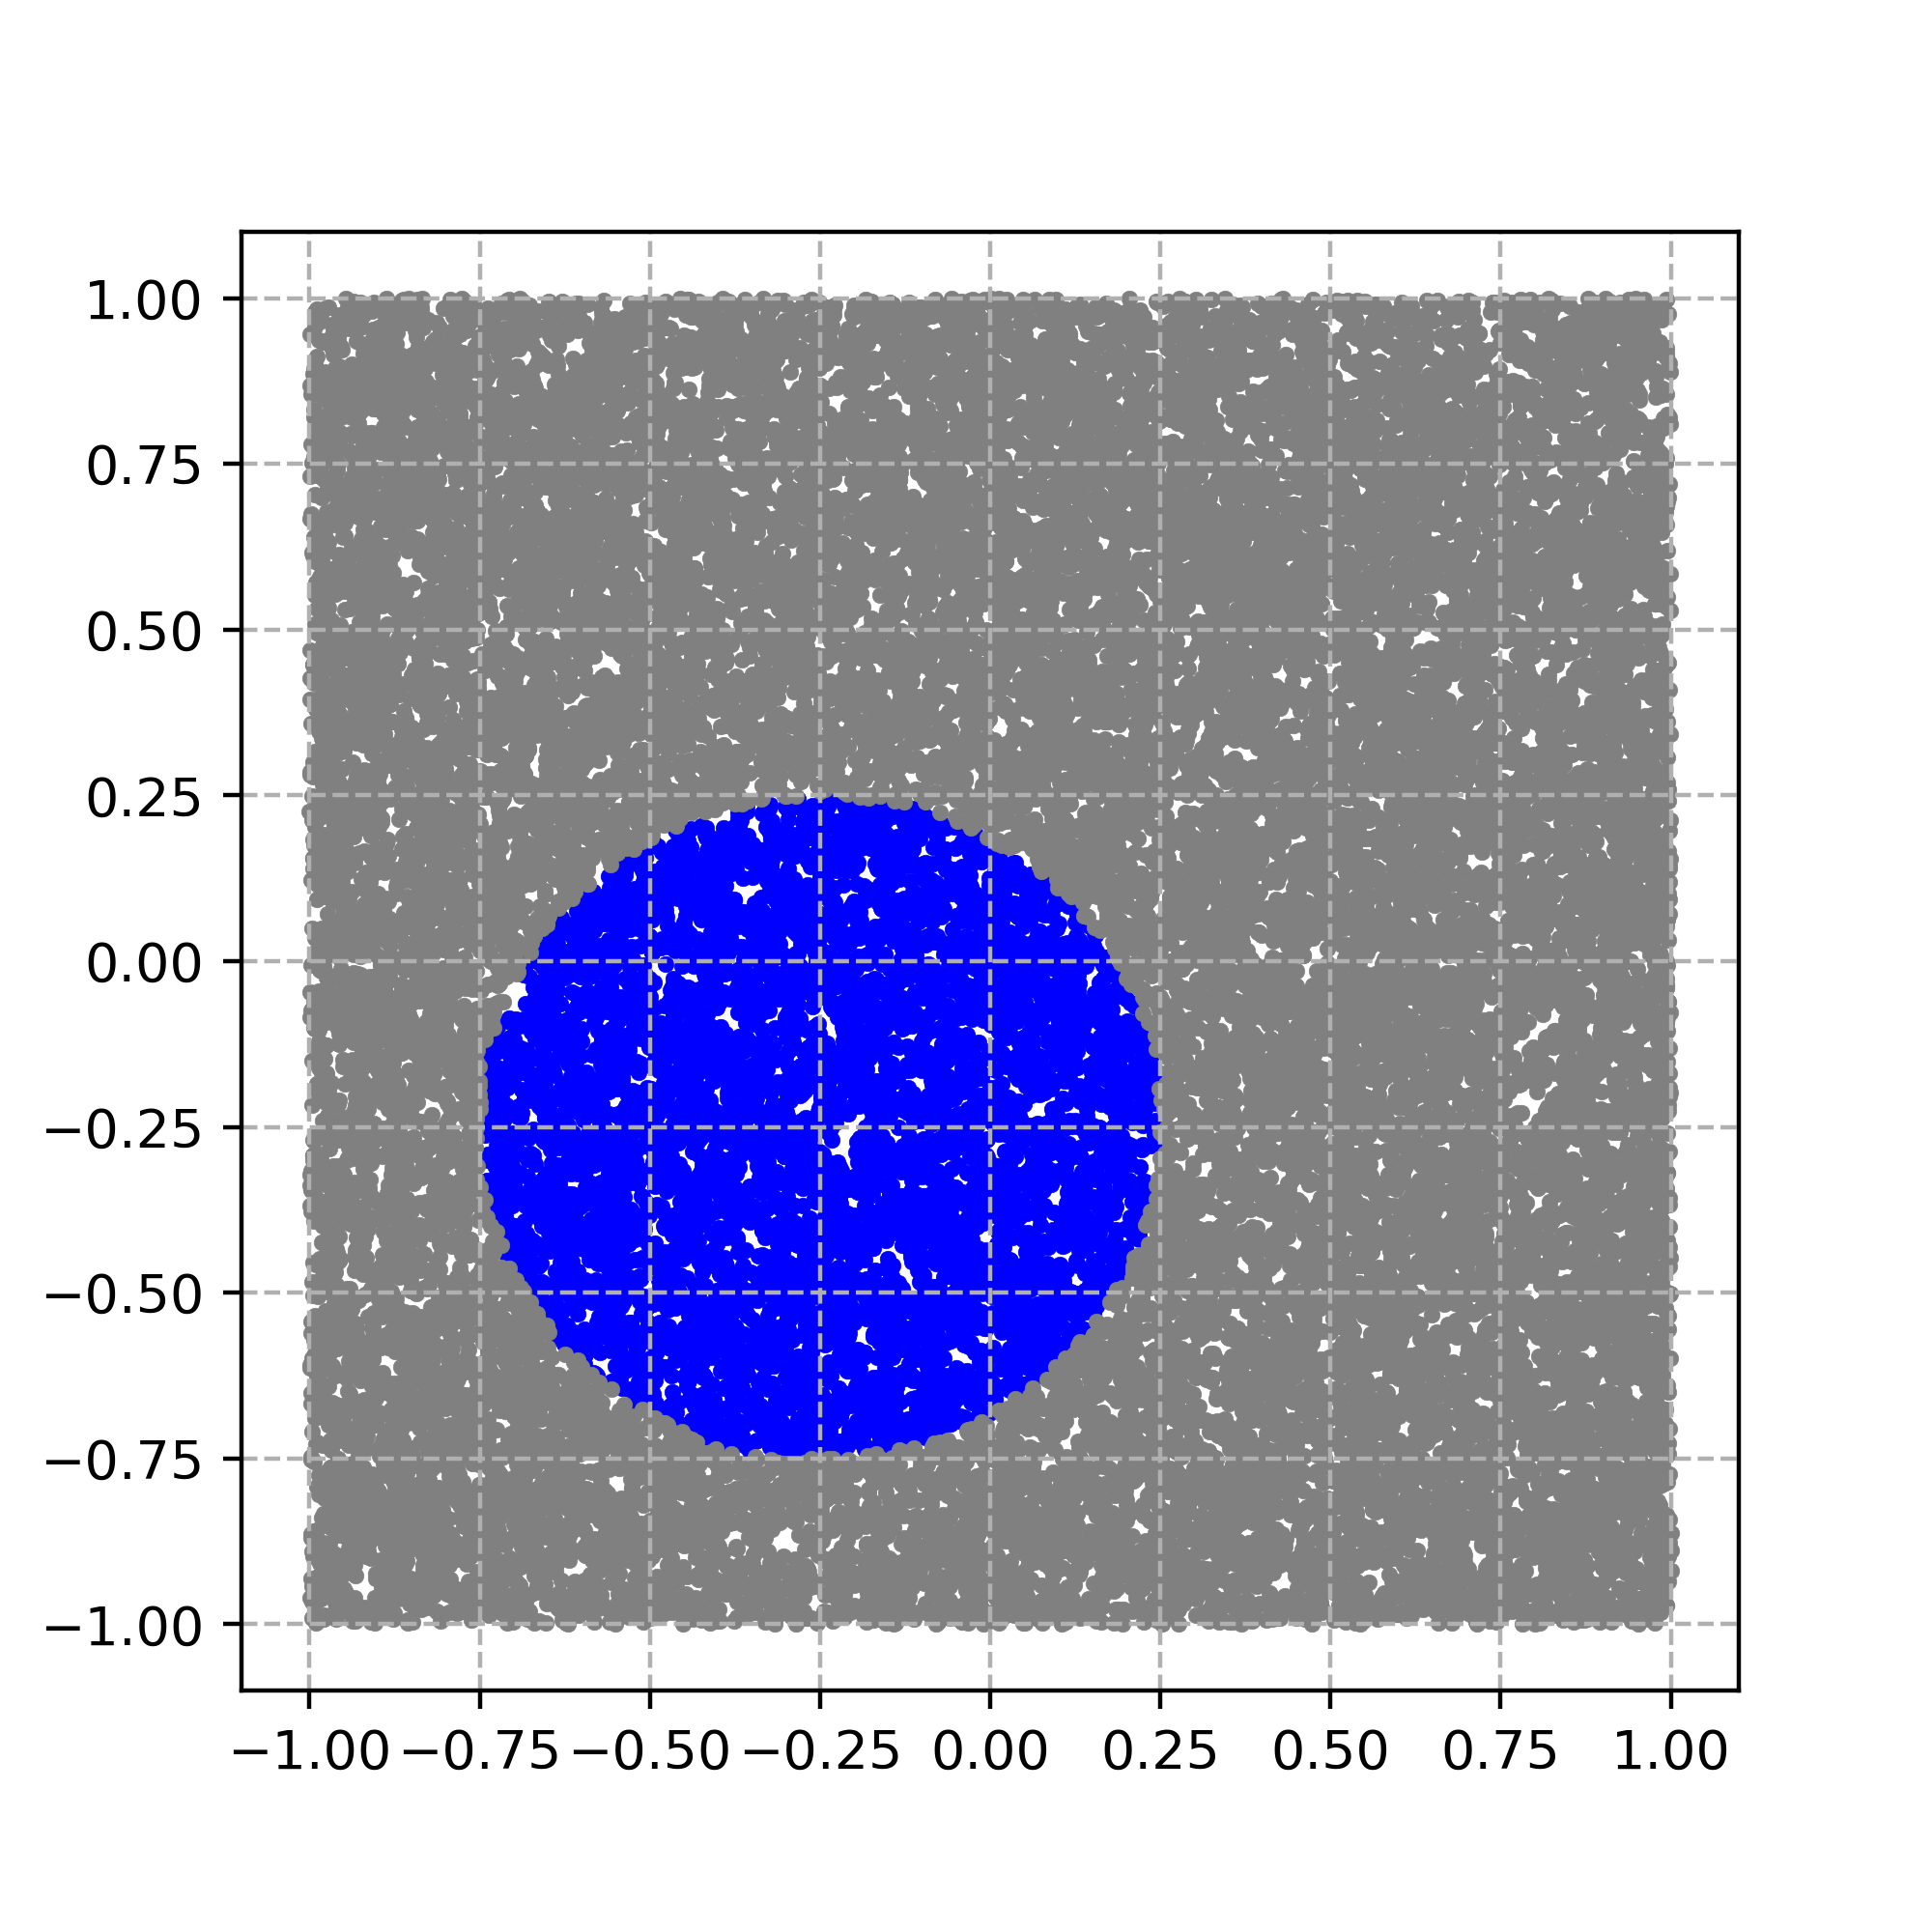
\includegraphics[width=\linewidth]{estimation4_2_30000.png}
				\caption{30000 points, $\pi= 3.1184$.}
			\end{subfigure}		
			\caption{$\pi$ estimation changing center of the circle, 2.}
			\label{fig::que4_2}
		\end{figure}    	
						
		As we see, our $\pi$ estimation is closer to the true value of $\pi$ the more samples we use regardless of where the center of the circle is. 
		
		%question 5
		\item
		What happens to the accuracy of the estimation when you increase the square size, or decrease the circle size? Is there an optimal ratio?
		
		The optimal ratio is when $l = d$ because this is the value for which the probability  of finding a point inside the circle is the highest; we “cover” the largest area when $l = d$. 
		
		As $d \rightarrow 0$, the rarer it is to encounter a point inside the circle; then, our estimation may be too poor.
		
		Additionally, from question 1, we may say that as $d \rightarrow 0$, the larger the quantity $l/d$ is for a fixed $l$. This means that although such a quantity counteracts the small value of our probability of finding a point inside the circle, our estimation is poor for small number of samples.
		
		Something similar happens if we increase the square's length and keep the circle's radius constant.
		
		When either the circle's length or the square's size is small with respect each other, it is rare to find a point falling inside the circle.
		
		\item
		Prove the Hellmann-Feynman theorem. 
		
		\begin{equation*}
		\begin{aligned}
			\dfrac{d}{d\lam} E(\lam) =
			\dfrac{d}{d\lam} \bra{  \Psi(\lam)} \hat{H}(\lam) \ket{ \Psi(\lam)} =\\
			 \bra{  \dfrac{d}{d\lam}  \Psi(\lam)} \hat{H}(\lam)  \ket{  \Psi(\lam)} +
			 \bra{ \Psi(\lam)} \dfrac{d}{d\lam} \hat{H}(\lam)  \ket{  \Psi(\lam)} + 
			 \bra{ \Psi(\lam)} \hat{H}(\lam) \ket{ \dfrac{d}{d\lam} \Psi(\lam)} = \\
			 E(\lam)
			 \left\{  
			 \braket{ \dfrac{d}{d\lam}\Psi(\lam) | \Psi(\lam)} + \braket{\Psi(\lam)| \dfrac{d}{d\lam} \Psi(\lam)}
			 \right\} + 	\bra{ \Psi(\lam)} \dfrac{d}{d\lam} \hat{H}(\lam)  \ket{  \Psi(\lam)}= \\
			 E(\lam) \dfrac{d}{d\lam} \braket{ \Psi(\lam) | \Psi(\lam)} 	+ \bra{ \Psi(\lam)} \dfrac{d}{d\lam} \hat{H}(\lam)  \ket{  \Psi(\lam)} = 
			 \bra{ \Psi(\lam)} \dfrac{d}{d\lam} \hat{H}(\lam)  \ket{  \Psi(\lam)} 
		\end{aligned}			
		\end{equation*}
	
	We assumed exact states and then we have: $ \hat{H}(\lam) \Psi(\lam) = E(\lam) \Psi(\lam)$; furthermore, we used $\braket{ \Psi(\lam) | \Psi(\lam)} = 1 \Rightarrow \dfrac{d}{d\lam} \braket{ \Psi(\lam) | \Psi(\lam)}$.
	
	\item
	Explain the Born-Oppenheimer approximation in your own words. You do not have to use any equations (but you may if you wish).
	
	All physical systems consist of molecules and as such, they are composed by electrons and nuclei. These particles interact with each other. The Born-Oppenheimer approximation assumes that the motion of electrons and nuclei can be separated. Such a model takes into account the fact that the electrons are much lighter that the nuclei (in terms of their masses),then they move faster and as such the nuclei are though as fixed, which leads to a wave-function expressed in terms of the position of electrons and nuclei. As a result, the wave function of a molecule can be written as a product of the electron's wave-function and the nuclei wave-function.	 
		 	
	\end{enumerate}
	
\end{document}    